\documentclass[11pt]{article}
\pdfoutput=1
\usepackage[margin=1in]{geometry} 

\usepackage{etoolbox}

\usepackage[round]{natbib}
\usepackage{array,amsmath,amsthm,amssymb,amsfonts,titling,bbm, titlesec, bm, physics, enumitem, accents, setspace, fancyhdr, natbib, geometry, pdflscape}
\usepackage{graphicx}
\usepackage{float}
\usepackage[font=footnotesize,labelfont=bf]{caption}
\usepackage{array}
\usepackage[title]{appendix}
\usepackage{afterpage}
\usepackage{listings}
\usepackage{prodint}
\usepackage{algorithm}
 \usepackage{booktabs}
\usepackage{multirow,booktabs}
\usepackage{subcaption}
\newlength{\continueindent}
\setlength{\continueindent}{2em}
\usepackage{etoolbox}
\usepackage{setspace}
\usepackage[dvipsnames]{xcolor}
\definecolor{mydarkgray}{rgb}{0.25,0.25,0.25}
\definecolor{Bleu}{RGB}{0,0,204}
\usepackage[hypertexnames=false]{hyperref}
\hypersetup{
colorlinks,
  citecolor=Bleu,
  linkcolor=Bleu,
  urlcolor=Bleu}

\usepackage{makecell}
\usepackage{tikz}
\def\checkmark{\tikz\fill[scale=0.4](0,.35) -- (.25,0) -- (1,.7) -- (.25,.15) -- cycle;} 
\newcommand{\hybridmark}{%
  \tikz[scale=0.4, line width=0.6pt]{
    % Checkmark shape
    \fill (0,.35) -- (.25,0) -- (1,.7) -- (.25,.15) -- cycle;
    % Diagonal slash over the right part
    \draw[line width=0.5pt] (0.4,0.55) -- (0.75,0.15);

  }%
}


\usepackage{tikz}
\usetikzlibrary{positioning, arrows.meta}

\usepackage{amssymb}
\usepackage{pifont}
\usepackage{booktabs}
\usepackage{multirow}

\lstdefinestyle{compact}{
    basicstyle=\ttfamily\small, % or \footnotesize
    lineskip=-0.5pt,
    aboveskip=0pt,
    belowskip=0pt,
    keepspaces=true,
    breaklines=true,
    columns=fullflexible
}

\doublespacing
 

\newcommand{\INPUT}{\item[\textbf{Input:}]}



\newcolumntype{P}[1]{>{\centering\arraybackslash}p{#1}}


\usepackage{amsmath}
\usepackage{amssymb}
\usepackage{amsthm,thmtools}
\usepackage{enumitem}
\usepackage{amsfonts}
\RequirePackage{algorithm}
\RequirePackage{algorithmic}
\usepackage{bm,upgreek}
\usepackage{mathrsfs}  
\bibliographystyle{plainnat}
 
\usepackage{calc}% http://ctan.org/pkg/calc
\usepackage{subcaption}
\usepackage{authblk}

\theoremstyle{plain}
\newtheorem{example}{Example}
\newtheorem{theorem}{Theorem}
\newtheorem{corollary}{Corollary}
\newtheorem{definition}{Definition}
\newtheorem{condition}{Condition}
\newtheorem{lemma}{Lemma}
\newtheorem{remark}{Remark}

\DeclareMathOperator{\E}{E}
\DeclareMathOperator{\sym}{Sym}
\newcommand{\matr}[1]{\bm{#1}}

\providecommand{\keywords}[1]
{
  \small
  \textbf{\textit{Keywords:}} #1
}
\usepackage[utf8]{inputenc}
\usepackage{textcomp}
\newcommand{\blue}[1]{{\color{purple}#1}}
\newcommand{\red}[1]{{\color{red}#1}}
\DeclareMathOperator*{\argmin}{argmin}
\DeclareMathOperator*{\argmax}{argmax}
\DeclareMathOperator*{\esssup}{ess\,sup}
\DeclareMathOperator*{\essinf}{ess\,inf}
\usepackage{xr-hyper}
\usepackage[capitalize,noabbrev]{cleveref}
\DeclareMathOperator*{\logit}{logit}
\DeclareMathOperator*{\expit}{expit}


\DeclareFontFamily{U}{jkpmia}{}
\DeclareFontShape{U}{jkpmia}{m}{it}{<->s*jkpmia}{}
\DeclareFontShape{U}{jkpmia}{bx}{it}{<->s*jkpbmia}{}
\DeclareMathAlphabet{\mathfrak}{U}{jkpmia}{m}{it}
\SetMathAlphabet{\mathfrak}{bold}{U}{jkpmia}{bx}{it}

\usepackage[hang,flushmargin]{footmisc}
\newcommand\blfootnote[1]{
  \begingroup
  \renewcommand\thefootnote{}\footnote{#1}%
  \addtocounter{footnote}{-1}%
  \endgroup
}

%\title{Automatic doubly robust inference
% for linear functionals \\
% via calibrated debiased machine learning}


\title{Doubly robust inference via calibration}

 
 % \title{Doubly robust inference via calibration}

%\title{Calibrated Debiased Machine Learning \\
 % for automatic doubly robust inference
 %of linear functionals}

\date{\today}

\author[1]{Lars van der Laan}
\author[1,2]{Alex Luedtke}
\author[2,1]{Marco Carone}
 
 
\affil[1]{\footnotesize Department of Statistics, University of Washington, Seattle, USA}
\affil[2]{\footnotesize Department of Biostatistics, University of Washington, Seattle, USA}
 
 \AtBeginEnvironment{algorithmic}{\normalsize}

\makeatletter
\newcommand*{\addFileDependency}[1]{% argument=file name and extension
  \typeout{(#1)}
  \@addtofilelist{#1}
  \IfFileExists{#1}{}{\typeout{No file #1.}}
}
\makeatother


\newcommand*{\myexternaldocument}[1]{%
    \externaldocument{#1}%
    \addFileDependency{#1.tex}%
    \addFileDependency{#1.aux}%
}

\myexternaldocument{main_JRSSB_appendix_revision}


% Requires:
 \usepackage{tikz}
 \usepackage{pgfplots}
 \pgfplotsset{compat=1.18}

 \usepackage{setspace}
\newcommand{\slightspacing}{\setstretch{1.175}}




\begin{document}

\allowdisplaybreaks
\maketitle

 

\singlespacing

\begin{abstract}
%Many statistical parameters, such as average treatment effects, can be represented as linear functionals of the outcome regression, a form that permits doubly robust estimation. . This holds under a partial orthogonality condition stating 
 
Doubly robust estimators are widely used for estimating average treatment effects and other linear summaries of regression functions. While consistency requires only one of two nuisance functions to be estimated consistently, asymptotic normality for linear functionals typically requires sufficiently fast convergence of both. We address this mismatch by showing that calibrating the nuisance
estimators within a doubly robust procedure yields doubly robust asymptotic
normality, provided that one nuisance estimator suitably captures the estimation error in
the other. We introduce a general framework, \emph{calibrated debiased machine learning} (calibrated DML), and propose a specific estimator that augments standard DML with a simple isotonic regression adjustment. Under a partial orthogonality condition, our theoretical analysis shows that the calibrated DML estimator remains asymptotically normal if either the regression or the Riesz representer of the functional is estimated sufficiently well, allowing the other to converge arbitrarily slowly or even inconsistently. We further propose a simple bootstrap method for constructing confidence intervals, enabling doubly robust inference without additional nuisance estimation. In a range of semi-synthetic benchmark datasets, calibrated DML reduces bias and improves coverage relative to standard DML.  Our method can be integrated into existing DML pipelines by adding just a few lines of code to calibrate cross-fitted estimates via isotonic regression.  

 

 
%In causal inference, many estimands of interest can be expressed as a linear functional of the outcome regression function; this includes, for example, average causal effects of static, dynamic and stochastic interventions. For learning such estimands, in this work, we propose novel debiased machine learning estimators that are doubly robust asymptotically linear, thus providing not only doubly robust consistency but also facilitating doubly robust inference (e.g., confidence intervals and hypothesis tests). To do so, we first establish a key link between calibration, a machine learning technique typically used in prediction and classification tasks, and the conditions needed to achieve doubly robust asymptotic linearity. We then introduce calibrated DML (C-DML), a unified framework for doubly robust inference, and propose a specific C-DML estimator that integrates cross-fitting, isotonic calibration, and debiased machine learning estimation. A C-DML estimator maintains asymptotic linearity when either the outcome regression or the Riesz representer of the linear functional is estimated sufficiently well, allowing the other to be estimated at arbitrarily slow rates or even inconsistently. We propose a simple bootstrap-assisted approach for constructing doubly robust confidence intervals. Our theoretical and empirical results support the use of C-DML  to mitigate bias arising from the inconsistent or slow estimation of nuisance functions and to ensure calibrated inferences.


% In this work, we correct this mismatch: we show that calibrating the nuisance estimators within a doubly robust procedure yields doubly robust inference.

% In this work, we show that calibrating the nuisance estimators within debiased machine learning (DML) yields inference that is itself doubly robust. We then propose a specific instantiation of \emph{calibrated DML} that simply augments standard DML with an isotonic regression adjustment. Our theoretical analysis shows that the calibrated DML estimator remains asymptotically linear if either the regression or the Riesz representer is estimated sufficiently well, allowing the other to converge arbitrarily slowly or even inconsistently. We further propose a bootstrap method for constructing confidence intervals. In a range of semi-synthetic benchmark datasets, calibrated DML reduces bias and improves coverage relative to uncalibrated DML.


% that simply augmenting standard debiased machine learning (DML) estimators with an isotonic regression adjustment

% Doubly robust estimators are widely used for estimating average causal effects and other linear functionals of regression functions. Although they are consistent if either the regression or an additional nuisance function is estimated consistently, constructing valid confidence intervals typically requires both nuisance functions to be estimated at sufficiently fast rates. In this work, we establish that simply calibrating nuisances when using a doubly robust estimator provides doubly robust inference properties. 

% % Our results support calibrating nuisances when using a doubly robust estimator.

% In this work, we propose novel debiased machine learning estimators that exhibit doubly robust asymptotic normality, extending double robustness from consistency to inference. We first establish a fundamental connection between the calibration of nuisance estimators---a technique typically used in prediction---and doubly robust asymptotic linearity. Building on this link, we introduce \emph{calibrated debiased machine learning} (calibrated DML), a unified framework for doubly robust inference, and propose a specific calibrated DML estimator that simply augments standard DML with an isotonic regression adjustment. Our theoretical analysis shows that the calibrated DML estimator remains asymptotically linear if either the regression or the Riesz representer is estimated sufficiently well, allowing the other to converge arbitrarily slowly or even inconsistently. We further propose a bootstrap method for constructing confidence intervals. In a range of semi-synthetic benchmark datasets, calibrated DML reduces bias and improves coverage relative to uncalibrated DML.



%In causal inference, many estimands of interest can be expressed as a linear functional of the outcome regression function; this includes, for example, average causal effects of static, dynamic and stochastic interventions. For learning such estimands, in this work, we propose novel debiased machine learning estimators that are doubly robust asymptotically linear, thus providing not only doubly robust consistency but also facilitating doubly robust inference (e.g., confidence intervals and hypothesis tests). To do so, we first establish a key link between calibration, a machine learning technique typically used in prediction and classification tasks, and the conditions needed to achieve doubly robust asymptotic linearity. We then introduce calibrated DML (C-DML), a unified framework for doubly robust inference, and propose a specific C-DML estimator that integrates cross-fitting, isotonic calibration, and debiased machine learning estimation. A C-DML estimator maintains asymptotic linearity when either the outcome regression or the Riesz representer of the linear functional is estimated sufficiently well, allowing the other to be estimated at arbitrarily slow rates or even inconsistently. We propose a simple bootstrap-assisted approach for constructing doubly robust confidence intervals. Our theoretical and empirical results support the use of C-DML  to mitigate bias arising from the inconsistent or slow estimation of nuisance functions and to ensure calibrated inferences.



\end{abstract}

  \keywords{debiasing, isotonic calibration,  double robustness, targeted learning, causal inference}



\doublespacing

 

\section{Introduction}

\subsection{Motivation}

 
 


 Nonparametric inference on the causal effects of dynamic and stochastic treatment interventions using flexible statistical learning techniques is a fundamental problem in causal inference. These inferential targets fall within a broader class of target parameters that can be expressed as linear functionals of the outcome regression, that is, the conditional mean of the outcome given treatment assignment and baseline covariates \citep{chernozhukov2018double, rotnitzky2021characterization, hirshberg2021augmented}. To achieve inference for such parameters, various debiased machine learning (DML) frameworks are available, including one-step estimation \citep{pfanzagl1985contributions, bickel1993efficient}, estimating equations and double machine learning \citep{robins1995analysis, robinsCausal, vanderlaanunified, DoubleML}, and targeted minimum loss estimation (TMLE) \citep{van2006targeted, vanderLaanRose2011}, and sieve-based estimators \citep{qiu2021universal, cho2024kernel}. When performing inference on linear functionals, debiased machine learning methods frequently produce estimators that demonstrate robustness against inconsistent or slow estimation of certain nuisance functions, a property known as double robustness \citep{bang2005doubly, smucler2019unifying}. For example, when estimating the average treatment effect (ATE),  doubly robust estimators remain consistent as long as either the outcome regression or the propensity score is consistently estimated, even if the other is inconsistently estimated. This robustness property extends more generally to linear functionals of the outcome regression, necessitating consistent estimation of only the outcome regression itself or the Riesz representer of the linear functional \citep{chernozhukov2018double, rotnitzky2021characterization}.

Extending the double robustness property of debiased machine learning
estimators to statistical inference is challenging. { \color{purple}By
\emph{double robustness for statistical inference}, we mean that valid
root-\(n\) inference remains possible when one nuisance function is estimated
consistently at a sufficiently fast rate, even if the other is not. In
standard debiased machine learning procedures, however, asymptotic normality
typically requires both the outcome regression and the Riesz representer to be
estimated consistently and sufficiently quickly, so that the product of their
estimation errors is \(o_p(n^{-1/2})\).} If this condition fails, desirable
properties such as asymptotic linearity, asymptotic normality, and
\(n^{1/2}\)-consistency can be lost, compromising the validity of inference
\citep{benkeser2017doubly}. In such
cases, standard confidence intervals and \(p\)-values can be invalid.
\textcolor{blue}{In practice, inconsistency may arise from model
misspecification (e.g., omitted interactions or nonlinearities) or
over-regularization of flexible learners, while slow convergence may occur when
the nuisance functions are intrinsically complex---for example, involving
nonsparse high-dimensional interactions or limited smoothness---so that
flexible learners cannot achieve fast rates.} One approach to achieving doubly
robust inference is to use parametric methods, such as maximum likelihood
estimation, to estimate the nuisance parameters. These methods exhibit model
double robustness, maintaining asymptotic linearity when at least one of the
nuisance parametric models is correctly specified
\citep{vermeulen2015bias, vermeulen2016data, shook2025double}. However, their
usefulness for nonparametric inference is limited by their reliance on strong
modeling assumptions, since in practice both models are often misspecified
\citep{kang2007demystifying}.
 
 
 
To overcome the limitations of parametric methods, several estimators exhibiting
\emph{sparsity double robustness}---a weaker form of model double robustness---have
been proposed \citep{avagyan2017honest, athey2018approximate, bradic2019sparsity,
bradic2019minimax, smucler2019unifying, tan2020model, zhang2021dynamic,
ghosh2022doubly, bradic2024high, baybutt2026doubly}. In high-dimensional
generalized linear models, \cite{avagyan2017honest} and
\cite{bradic2019sparsity, bradic2019minimax} introduced doubly robust
\(\ell_1\)--regularized estimators of the ATE that are asymptotically normal
when either the outcome regression or propensity score is sufficiently sparse,
allowing misspecification of one nuisance model. Relatedly,
\cite{athey2018approximate} and \cite{tan2020model} proposed singly robust
estimators that are robust to misspecification of the outcome regression,
assuming sufficient sparsity of the propensity score. A key limitation of these
approaches is their reliance on strong sparsity assumptions, which may fail in
practice. \cite{bradic2019minimax} study doubly robust inference under
approximate sparsity, but still impose a product-rate condition on the
approximation errors of both nuisance functions with respect to the chosen
basis dictionary (Assumption~2). \cite{smucler2019unifying} develop a unifying
\(\ell_1\)-regularization framework for sparse doubly robust estimation,
accommodating model misspecification by allowing the nuisance estimators to
converge to approximately sparse, potentially misspecified limits at a sufficiently fast rate. {\color{purple}
For the ATE, \cite{liu2023root} relax sparsity requirements on misspecified
limits by assuming sparsity only for the consistently estimated nuisance, albeit
at the cost of irregularity and loss of efficiency. Finally, these methods are not
learner-agnostic: they are largely tied to \(\ell_1\)-regularized generalized
linear models for the nuisance functions, which limits their ability to
leverage modern machine-learning methods.}
 
 
 
By contrast, the line of work initiated by \cite{van2014targeted} and further developed by \cite{benkeser2017doubly} provides a learner-agnostic debiasing framework---based on targeted maximum likelihood estimation (TMLE) \citep{vanderLaanRose2011}---for doubly robust inference with nuisance functions estimated using generic machine learning methods. Under suitable conditions, the resulting estimators are \emph{doubly robust asymptotically linear} (DRAL): they remain asymptotically linear, and hence asymptotically normal under standard conditions, even if one nuisance estimator is inconsistent, provided the other is estimated sufficiently well (i.e., at rate \(o_p(n^{-1/4})\)). Concretely, for the  ATE, if \(\pi_n\) and \(\mu_n\) estimate the propensity score \(\pi_0\) and outcome regression \(\mu_0\), then a DRAL estimator can remain asymptotically linear under the \emph{best-rate} condition that $\|\pi_n - \pi_0\| = o_p(n^{-1/4})$ or $
\|\mu_n - \mu_0\| = o_p(n^{-1/4}),$
whereas rate double robustness imposes the more stringent product-rate condition $\|\mu_n - \mu_0\| \, \|\pi_n - \pi_0\| = o_p(n^{-1/2}).$
For the ATE, these methods iteratively update initial propensity score and
outcome regression estimates using low-dimensional (often one-dimensional)
regressions that enforce moment conditions and debias the cross-product
remainder in the asymptotic expansion. This approach has since been extended to nonparametric inference for mean outcomes under informative missingness \citep{diaz2017doubly}, counterfactual survival curves \citep{diaz2019statistical}, and semiparametric inference for the ATE in partially linear regression models \citep{dukes2024doubly}.


 


The TMLE-based framework for doubly robust inference has some limitations.
First, the iterative debiasing procedure is difficult to study theoretically
and can be computationally demanding to implement, posing challenges for its
application to large-scale data or complex data structures. While \cite{bonvini2024doubly} proposed a non-iterative, nonparametric DRAL
estimator of the ATE based on higher-order influence functions, their procedure
requires careful tuning of bivariate kernel-smoothing parameters, for which
practical guidance remains limited. Second, when considering new
parameters of interest, a new debiasing algorithm must be derived on a
case-by-case basis, requiring careful analysis of the relevant remainder terms
and novel targeting constructions. To date, there is no unified, learner-agnostic approach to doubly robust
inference for a generic linear functional of the outcome regression. Finally, the available guarantees are mainly designed for
one-sided misspecification and do not strengthen inference when both nuisance
estimators are consistent but one converges too slowly for the product-rate
condition to hold. Indeed, they typically assume that both nuisance estimators converge to their
(possibly misspecified) limits at rate \(o_p(n^{-1/4})\).



\subsection{Contributions of this work}

  \begin{figure}[tb]
\centering
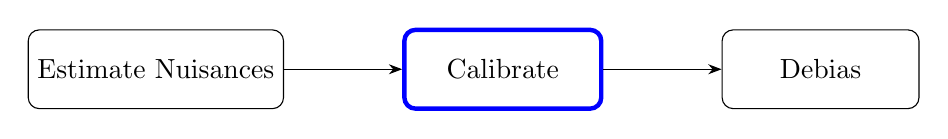
\begin{tikzpicture}[node distance=0.8cm and 1.5cm, every node/.style={draw, rounded corners, align=center, minimum height=1cm, minimum width=2.5cm}, >=Stealth]

% Calibrated DML
\node (estimate_cal) {Estimate Nuisances};
\node (calibrate_cal) [right=of estimate_cal, draw=blue, ultra thick] {Calibrate};
\node (debias_cal) [right=of calibrate_cal] {Debias};

\draw[->] (estimate_cal) -- (calibrate_cal);
\draw[->] (calibrate_cal) -- (debias_cal);

\end{tikzpicture}
\caption{We show \textbf{calibrating the nuisances} before debiasing ensures doubly robust asymptotic normality.}
\label{fig:dml_flowchart}
\end{figure}


 
We develop new methods for doubly robust inference on linear functionals of the outcome regression. Our goal is to construct DRAL estimators that permit valid inference when one of the two nuisance functions is estimated arbitrarily slowly or even inconsistently, provided that at least one nuisance converges at an \(o_p(n^{-1/4})\) rate. We first establish a link between calibration, a technique typically used in prediction and classification tasks \citep{zadrozny2001obtaining, niculescu2005predicting}, and doubly robust asymptotic linearity. We then introduce a general framework, \emph{calibrated debiased machine learning} (calibrated DML). {\color{purple} As outlined in Figure~\ref{fig:dml_flowchart}, calibrated DML begins with standard cross-fitted estimates of the outcome regression and Riesz representer, obtained using any machine learning algorithm. It then adds a single post-hoc step: each nuisance estimator is \emph{calibrated} by fitting a one-dimensional map from its fitted values to its target using, e.g., isotonic regression \citep{barlow1972isotonic}. We show that this calibration step enforces an appropriate empirical orthogonality between the nuisance errors, which enables a one-step debiased estimator to achieve doubly robust asymptotic linearity. This is achieved under a partial orthogonality condition comparable to those
assumed in prior work on learner-agnostic doubly robust inference, including
\cite{van2014targeted,benkeser2017doubly,diaz2017doubly,dukes2024doubly,bonvini2024doubly}.}  Confidence intervals can be constructed using the closed-form influence function of the calibrated DML estimator, without requiring knowledge of which nuisance estimators converge sufficiently quickly. We show that no correction is needed to the standard influence-function-based variance estimator when both nuisance estimators are consistent for the true nuisances, even if one converges arbitrarily slowly. When one nuisance may be inconsistently estimated, we propose a computationally efficient bootstrap-assisted procedure that avoids the additional nuisance estimation required in \cite{van2014targeted} and related approaches, {\color{purple} and remains valid under the same nuisance-rate conditions. }


 

 



%We aim to derive doubly robust inferential procedures for linear functionals of the outcome regression. Specifically, these procedures should facilitate valid inference even when one nuisance estimator converges to its intended target arbitrarily slowly or even inconsistently. We introduce a novel estimation framework, which we refer to as \emph{calibrated DML}, that allows for the construction of DRAL estimators and confidence intervals that provide doubly robust inferences. To accomplish this, we rely on cross-fitted estimators of the outcome regression and Riesz representer obtained using any generic supervised learning algorithms. Within the calibrated DML procedure, calibrated nuisance estimators may be constructed, for example, using a generalization of isotonic calibration --- a technique commonly used in prediction and classification tasks \citep{zadrozny2001obtaining, niculescu2005predicting, van2023causal}---based on loss functions tailored for the task at hand. These calibrated estimators are then used to create a calibrated one-step debiased estimator, which we refer to as a calibrated DML estimator. 


\begin{table}[tb]
\centering
\caption{
Properties of G-computation plug-in, IPW, AIPW and calibrated DML (proposed approach) estimators of the ATE when nuisances are estimated using machine learning,  in settings where only the propensity score vs. only the outcome regression vs. both nuisances are estimated well {\color{purple} (i.e., consistently and at a rate faster than $n^{-1/4}$)}. Report whether each estimator is \textbf{consistent}, asymptotically \textbf{normal} at root-sample size rate, and nonparametric \textbf{efficient}. \\
($\ast$) Our estimator is efficient if one nuisance is estimated well), provided the other is estimated consistently (at any rate).
}
\label{tab:calibration_summary}
\resizebox{\textwidth}{!}{%
\begin{tabular}{l@{\hskip 6pt}!{\vrule width 0.8pt}@{\hskip 6pt}
>{\centering\arraybackslash}m{1.7cm}
>{\centering\arraybackslash}m{1.8cm}
>{\centering\arraybackslash}m{1.7cm}|
>{\centering\arraybackslash}m{1.7cm}
>{\centering\arraybackslash}m{1.8cm}
>{\centering\arraybackslash}m{1.7cm}|
>{\centering\arraybackslash}m{1.7cm}
>{\centering\arraybackslash}m{1.8cm}
>{\centering\arraybackslash}m{1.7cm}
}
% Top row: no vertical rule
\multicolumn{1}{c}{} & \multicolumn{3}{c}{\makecell{only propensity score \\ estimated well}} 
& \multicolumn{3}{c}{\makecell{only outcome regression \\ estimated well}} 
& \multicolumn{3}{c}{\makecell{both nuisance functions \\ estimated well}} \\[.175in]
\textbf{estimator} 
& \textbf{consistent} & \textbf{normal} & \textbf{efficient}
& \textbf{consistent} & \textbf{normal} & \textbf{efficient}
& \textbf{consistent} & \textbf{normal} & \textbf{efficient} \\
\midrule\midrule
G-computation      
& {\color{darkgray}--} & {\color{darkgray}--} & {\color{darkgray}--} 
& \checkmark & {\color{mydarkgray}\texttimes} & {\color{mydarkgray}\texttimes} 
& {\color{darkgray}--} & {\color{darkgray}--} & {\color{darkgray}--} \\
%+ calibration             
%& {\color{darkgray}--} & {\color{darkgray}--} & {\color{darkgray}--} 
%& \checkmark & \checkmark & {\color{mydarkgray}\texttimes} 
%& {\color{darkgray}--} & {\color{darkgray}--} & {\color{darkgray}--}  \\
IPW          
& \checkmark & {\color{mydarkgray}\texttimes} & {\color{mydarkgray}\texttimes} 
& {\color{darkgray}--} & {\color{darkgray}--} & {\color{darkgray}--} 
& {\color{darkgray}--} & {\color{darkgray}--} & {\color{darkgray}--} 
\\
%+ calibration                
%& \checkmark & \checkmark & {\color{mydarkgray}\texttimes} 
%& {\color{darkgray}--} & {\color{darkgray}--} & {\color{darkgray}--} 
%& {\color{darkgray}--} & {\color{darkgray}--} & {\color{darkgray}--} 
AIPW                  
& \checkmark & {\color{mydarkgray}\texttimes} & {\color{mydarkgray}\texttimes}
& \checkmark & {\color{mydarkgray}\texttimes} & {\color{mydarkgray}\texttimes} 
& \checkmark & \checkmark & \checkmark \\
\textbf{Calibrated DML} (ours)              
& \checkmark & \checkmark  & \checkmark {\small $\ast$}
& \checkmark & \checkmark  & \checkmark {\small $\ast$}
& \checkmark & \checkmark & \checkmark \\
\bottomrule
\end{tabular}%
}
\end{table}

 
 {\color{purple} Table~\ref{tab:calibration_summary} summarizes the properties of a specific implementation of calibrated DML in the well-studied setting of ATE estimation. This implementation employs isotonic regression for calibration and a cross-fitted augmented inverse probability weighted (AIPW) estimator for debiasing. Compared to the standard AIPW estimator, calibrated DML remains asymptotically normal under weaker convergence requirements: it suffices that one nuisance be consistently estimated at an $o_p(n^{-1/4})$ rate (the other may be inconsistent). It is efficient when \emph{both} nuisances are consistently estimated (with at least one attaining an $o_p(n^{-1/4})$ rate). Calibrated DML can yield even larger improvements over non-doubly robust estimators based on the G-computation formula or inverse probability weighting (IPW), since these estimators are neither doubly robust nor generally asymptotically normal under flexible nuisance estimation.}



 


%\emph{The proposed procedure can simply be implemented using standard DML procedures but with one key intermediate step added: the nuisance function estimators must be calibrated before the desired DML estimator is computed.} For inference on counterfactual means or the ATE, an augmented inverse probability weighted (AIPW) estimator in which the cross-fitted propensity score and outcome regression estimators are calibrated using isotonic calibration provides an example of a calibrated DML estimator; we refer to the resulting procedure as the calibrated AIPW (C-AIPW) estimator. In Table \ref{tab:calibration_summary}, we summarize properties of the C-AIPW estimator in contrast to standard estimators, including the plug-in estimator based on the G-computation formula, the inverse probability weighted (IPW) estimator, and the uncalibrated AIPW estimator. More generally, we derive the closed-form influence function of our proposed estimators, allowing us to construct confidence intervals without needing to know which, if any, of the nuisance functions is possibly estimated too slowly or inconsistently. To avoid the estimation of additional nuisance functions that arise in \cite{van2014targeted} and related works, we propose an automated bootstrap-assisted procedure for doubly robust inference, which is both computationally efficient and valid as long as at least one of the nuisance estimators is consistent at a sufficiently fast rate. 


 Our approach is motivated by the DRAL estimators of the ATE proposed by \citet{van2014targeted} and developed further in subsequent work \citep{benkeser2017doubly, diaz2017doubly, diaz2019statistical, dukes2024doubly}. We share the objective of constructing nuisance estimators that achieve doubly robust asymptotic linearity by solving certain score equations, but our strategy and implementation differ substantially, even for the ATE. In particular, our approach is a non-iterative and computationally efficient two-step procedure that can be implemented using commonly available isotonic regression software. Moreover, our method does not depend on the specific form of the linear functional; rather, it requires initial nuisance estimators and black-box access to an empirical estimator of the functional. { \color{purple} We share with \cite{benkeser2017doubly} the property that our estimator admits Wald-type inference based on a closed-form influence function, without requiring the analyst to know which nuisance is correctly specified. Unlike \cite{benkeser2017doubly}, however, our proposed bootstrap-assisted inference procedure avoids estimating the additional nuisance components that appear in the closed-form influence function, which can simplify implementation and potentially improve finite-sample performance. } Finally, our theoretical results refine those of prior work by showing that our estimator achieves asymptotic linearity not only under consistent estimation of one nuisance function alone, but also when both nuisance functions are estimated consistently and one is estimated too slowly.



 

  
\subsection{Related work}
 
\label{sec:relatedwork}
 

 


\medskip  \noindent \emph{Calibration in causal inference.}  Prior work has studied the finite-sample benefits of calibrating propensity score estimates in IPW and AIPW estimators of the ATE \citep{gutman2022propensity, deshpande2023calibrated, ballinari2024improving, van_der_Laan2024stabilized, rabenseifner2025calibrationstrategiesrobustcausal}. These studies focus primarily on calibrating a single nuisance function---the propensity score---for a single parameter (the ATE), and they do not provide theoretical justification beyond the observation that calibration can reduce nuisance estimation error. We extend this line of work by showing that, for general linear functionals, calibrating \emph{both} the outcome regression and the Riesz representer is key for further debiasing (in finite samples and asymptotically) and for constructing DRAL estimators. {\color{purple} More broadly, our work shows that calibration can yield asymptotic guarantees and relax nuisance-rate requirements, rather than serving only to improve the finite-sample quality of nuisance estimators. In the special case of the ATE, we find that calibrating the outcome regression can reduce finite-sample bias and remove certain asymptotic bias terms.}


 

 

 

 \medskip\noindent \emph{Sparsity double robustness.} {\color{purple}
Our calibration-based approach to doubly robust inference is closely related to
the literature on (approximate) sparsity-based doubly robust inference
discussed in the Introduction \citep{athey2018approximate, bradic2019minimax,
smucler2019unifying, tan2020model, liu2023root}. Methodologically, our approach
enforces one-dimensional orthogonality conditions on nuisance errors via
calibration (see \eqref{eqn::orthogonaloutcome}--\eqref{eqn::orthogonalRiesz}),
whereas sparsity-based methods typically enforce high-dimensional moment
conditions. In particular, when the nuisances are estimated by
\(\ell_1\)-regularized empirical risk minimization over linear classes, the
Karush--Kuhn--Tucker (KKT) conditions yield approximate empirical orthogonality
over suitable linear subspaces (see, e.g., \citealp[Eq.~15]{tan2020model};
\citealp[Sec.~2.1]{bradic2019sparsity}; \citealp[Sec.~4.1]{smucler2019unifying}).
We also note a terminology difference: \cite{tan2020model}, \cite{liu2023root},
and related work use ``calibration'' in the survey-sampling sense, referring to
adjustments that enforce moment conditions \citep{deville1992calibration},
whereas we use ``calibration'' in the machine-learning sense to mean
mean-unbiasedness conditional on the model's own prediction, a one-dimensional
objective. The analogous high-dimensional goal is closely related to
\emph{multi-accuracy}; see \citealp{roth2022uncertain}. We discuss these
differences in more detail in Appendix~\ref{appendix:relatedwork}.


Our closest comparison is \cite{liu2023root}: both methods apply a post-hoc
correction, but \cite{liu2023root} solve a high-dimensional moment-matching
problem built on preliminary \(\ell_1\)-regularized generalized linear models,
whereas we use a one-dimensional calibration step and allow arbitrary
user-supplied first-stage learners. The guarantees differ accordingly: we show
that one-dimensional calibration suffices for DRAL under a
partial-orthogonality condition (the upcoming \ref{cond:ortho}) on the nuisances, whereas \cite{liu2023root}
rely on sparsity conditions tailored to their high-dimensional setting and
require an auxiliary sample (e.g., via sample splitting) and careful tuning.
Efficiency guarantees also differ: our calibrated DML estimators are
semiparametrically efficient when both nuisances are consistent and at least
one converges faster than \(n^{-1/4}\) (Table~\ref{tab:calibration_summary}),
whereas \cite{liu2023root} do not generally establish semiparametric
efficiency. In contrast, related works, such as \cite{bradic2019minimax} and \cite{smucler2019unifying}, establish
efficiency under additional approximate sparsity assumptions on the (potentially
misspecified) limit of the slower nuisance estimator.
}

\medskip\noindent \emph{Higher-order influence functions and undersmoothing.} {\color{purple}
Higher-order influence function (HOIF) estimators \citep{robins2008higher, liu2017semiparametric}
use higher-order bias corrections to relax the nuisance-rate requirements of
first-order doubly robust methods, and can yield asymptotically valid and
efficient inference even when nuisance estimators fail to satisfy the usual
\(o_p(n^{-1/2})\) product-rate condition. Related robustness to slow nuisance rates can also be obtained without explicit HOIF-based corrections by combining sample splitting with undersmoothing
\citep{newey2018cross, mcgrath2022nuisance, mcclean2024double}. While HOIF methods can accommodate
flexible first-stage machine-learning estimators, their higher-order bias
correction typically relies on smoothness and approximability assumptions
(often H\"older-type) to control higher-order remainders, and it introduces
additional tuning parameters---such as the choice of basis functions,
truncation order, sieve dimension, or bandwidth---for which practical guidance
is limited. Consequently, HOIF estimators can be substantially more complex to implement
and tune, and may degrade in high dimensions due to sensitivity to these
assumptions and choices. For the expected conditional covariance parameter,
\cite{bonvini2024doubly} establish a connection between the learner-agnostic
doubly robust inference approaches of \cite{benkeser2017doubly} and related work and HOIF
estimators: they propose HOIF-based DRAL estimators that use the nuisance
estimates \((\mu_n,\alpha_n)\) as a bivariate dimension reduction and derive
guarantees under conditions comparable to those in our work and related
TMLE-based procedures \citep{benkeser2017doubly}. By contrast, calibrated DML
performs a higher-order bias correction via a simple post-hoc calibration step,
requiring no additional nuisance estimation beyond first-order methods; moreover,
isotonic calibration is tuning-free.}
  
%Related robustness to slow nuisance rates can also be obtained without explicit HOIF-based corrections by combining sample splitting with undersmoothing
%\citep{newey2018cross, mcgrath2022nuisance, mcclean2024double}. In particular,
%double cross-fitting estimates nuisance components on independent folds, so that
%leading remainder terms involve products of nuisance \emph{biases} rather than
%products of root mean squared errors. By reducing bias, undersmoothing can
%therefore permit valid inference under slower-than-usual nuisance rates. These
%approaches still require nuisance consistency, offer limited practical guidance
%for undersmoothing, and double cross-fitting reduces the effective sample size
%available for nuisance training, which can harm finite-sample performance.}
 
  

% Finally, for efficiency, our calibrated DML estimators require consistent estimation of both nuisance functions, with at least one converging faster than $n^{-1/4}$, as summarized in Table~\ref{tab:calibration_summary}. In contrast, \cite{liu2023root} appear to require strong (approximate) sparsity assumptions on both nuisance functions to attain efficiency (see Remark 3 of \cite{liu2023root}).
 
 
 

 
\medskip\noindent \emph{Organization.} This paper is organized as follows. In Section \ref{section::startsetup}, we introduce the class of regression functionals we consider and provide background on a standard rate-doubly-robust debiased estimator. In Section \ref{section:prelimDRinference}, we formulate the problem of doubly robust inference, introduce a model-agnostic linear expansion for the bias of one-step debiased estimators, and demonstrate how further debiasing of nuisances can be employed to construct DRAL estimators. In Section \ref{section::proposedestimator}, we present a novel link between nuisance estimator calibration and the doubly robust inference properties of debiased machine learning estimators, use this link to build our general calibrated DML framework, and propose a calibrated DML estimator based on isotonic regression with accompanying bootstrap-based confidence intervals. In Section \ref{section::theory}, we establish the theoretical properties of our proposed calibrated DML estimators and confidence intervals. Finally, we empirically investigate the performance of calibrated DML in Section \ref{section::experiments} and provide concluding remarks in Section \ref{section::conclusion}.



 

 \section{Problem setup}
 
 \label{section::startsetup}
 
\subsection{Data structure and target parameter}
\label{section::setup}
 
In this section, we introduce the data structure and the class of regression
functionals under consideration, along with their semiparametric efficiency
bound. In the next subsection, we review the standard one-step debiased
estimator and its rate double robustness property. We then explain why rate
double robustness alone is insufficient for doubly robust inference, thereby
motivating our objective of doubly robust asymptotic linearity in
Section~\ref{section:prelimDRinference}.




Suppose we observe an i.i.d.\ sample $Z_1,\ldots,Z_n$ of
$Z=(W,A,Y)\sim P_0$, where $W\in\mathcal W\subset\mathbb R^d$ are baseline
covariates, $A\in\mathcal A\subset\mathbb R^p$ is a treatment, and $Y\in\mathbb R$
is a bounded outcome. For any distribution $P$, let
$\mu_P(a,w) := E_P\{Y \mid A=a, W=w\}$ denote the outcome regression and
$P f := \int f(z)\,dP(z)$ for any integrable function $f$. We denote by
$P_{0,A,W}$ the marginal distribution of $(A,W)$ under $P_0$, by
$\mathcal H := L^2(P_{0,A,W})$ the corresponding Hilbert space of
square-integrable functions on $\mathcal A \times \mathcal W$ with inner product
$\langle \mu_1,\mu_2\rangle := \int \mu_1(a,w)\mu_2(a,w)\,P_{0,A,W}(da,dw)$, and
by $\|\cdot\|$ the induced norm. For general $P$, we write
$\|\mu\|_P := \{\int \mu(a,w)^2\,P_{A,W}(da,dw)\}^{1/2}$, where $P_{A,W}$ is the
marginal law of $(A,W)$ under $P$. Let $\mathcal{M}$ be a nonparametric model containing $P_0$.
To simplify notation, we write \(S_0\) for any summary \(S_{P_0}\) of the true
distribution \(P_0\).


%satisfying a variation independence property: for every \( \mu \in \mathcal{H} \), there exists \( P \in \mathcal{M} \) such that \( P_{A,W} = P_{0,A,W} \) and \( \mu_P = \mu \). To simplify notation, we write $S_0$ for any summary $S_{P_0}$ of the true distribution $P_0$.


 



%Suppose that we have at our disposal a sample of $n$ independent and identically distributed observations, $Z_1, \dots, Z_n$, of the data structure $Z := (W,A,Y)$ drawn from a probability distribution $P_0$. In this data structure, $W \in \mathcal{W} \subset \mathbb{R}^d$ is a vector of baseline covariates, $A \in \mathcal{A} \subset \mathbb{R}^p$ is a potentially multi-valued treatment assignment, and $Y \in \mathbb{R}$ is a bounded outcome. For any given distribution $P$, we define pointwise the outcome regression $\mu_P(a,w):= E_P(Y \,|\,  A = a , W = w)$ for any realization $(a,w)$ in the $P$--support of $(A,W)$, and denote by $Pf$ the integral $\int f(z)dP(z)$ for any $P$--integrable real-valued function $f$. When $\mathcal{A}$ is discrete, we also define the (generalized) propensity score $\pi_P(a |  w) := P(A=a\,|\,  W =w)$. We denote by $P_{0,A,W}$ the marginal distribution of $(A, W)$ induced by $P_0$, by  $\mathcal{H}:=L^2(P_{0,A,W})$ the Hilbert space of real-valued $P_{0,A,W}$--square  integrable functions on $\mathcal{A}\times\mathcal{W}$ equipped with the inner product $(\mu_1, \mu_2) \mapsto \langle \mu_1,\mu_2\rangle:=\iint \mu_1(a,w)\mu_2(a,w)P_{0,A,W}(da,dw)$, and by $\|\cdot\|$ the induced norm. Similarly, for any given distribution $P$, we denote by $\|\mu\|_P$ the norm $\{\iint \mu(a,w)^2P_{A,W}(da,dw)\}^\frac{1}{2}$ of $\mu$, where $P_{A,W}$ is the marginal distribution of $(A,W)$ induced by $P$. We suppose that $\mathcal{M}$ is a locally nonparametric model for $P_0$ satisfying the following variation independence property: for every $\mu \in \mathcal{H}$, there exists $P \in \mathcal{M}$ such that $P_{A,W} = P_{0,A,W}$ and $\mu_{P} = \mu$. To simplify notation, we write $S_0$ for any summary $S_{P_0}$ of the true data-generating distribution $P_0$.


 
Our objective is to develop doubly robust nonparametric inference for a
linear summary \(\tau_0 := \psi_0(\mu_0)\) of the outcome regression \(\mu_0\),
where \(\psi_0 : \mathcal{H} \to \mathbb{R}\) is an \(L^2\)-continuous linear
functional. We allow the functional of interest to depend on the unknown
data-generating distribution \(P_0\), viewing \(\psi_0\) as the evaluation at
\(P_0\) of a smooth mapping \(P \mapsto \psi_P\) defined on the statistical
model \(\mathcal{M}\). As illustrated at the end of this subsection, many
parameters take this form, including average causal effects; this framework
also subsumes the class of continuous linear functionals studied in
\cite{chernozhukov2022automatic,bradic2019minimax}.
 

We impose the following smoothness conditions on the mapping
\((P,\mu)\mapsto \psi_P(\mu)\), which are sufficient for pathwise
differentiability of the composite parameter \(\Psi : P \mapsto \psi_P(\mu_P)\)
at \(P_0\). For each \(P\in\mathcal{M}\), we view \(\psi_P\) as a bounded linear
functional on the normed space \((\mathcal{H}, \|\cdot\|_{L^2(P_{0,A,W})})\),
equipped with the corresponding operator norm.



\begin{enumerate}[label=\bf{A\arabic*)}, ref={A\arabic*}, series = introcond]
    \item \textit{(linearity and boundedness)}\label{cond::linear}  it holds that $\psi_0(c\mu_1 + \mu_2) = c\psi_0(\mu_1) + \psi_0(\mu_2)$ for each $\mu_1,\mu_2\in \mathcal{H}$ and $c\in\mathbb{R}$ and that $\sup_{\mu \in \mathcal{H}\backslash \{0\}} |\psi_0(\mu)|/\|\mu\| < \infty$;
    \item \textit{(Hellinger continuity)} \label{cond::continuous}  $P \mapsto \psi_P$ is a continuous map at $P_0$ with domain $\mathcal{M}$ equipped with the Hellinger distance and codomain $\{\psi_P: P \in \mathcal{M}\}$ equipped with the operator norm;  
    \item \textit{(pathwise differentiability)}\label{cond::pathwise} for each $\mu \in \mathcal{H}$, $P \mapsto \psi_P(\mu)$ is pathwise differentiable at $P_0$ relative to $\mathcal{M}$ with efficient influence function $\phi_{0, \mu} \in L^2_0(P_0)$.
\end{enumerate} 


A key object associated with a continuous linear functional is its Riesz
representer, which plays a central role in debiasing and in the construction of
asymptotically linear estimators of \(\tau_0\) (see \cite{williams2025riesz} for an
accessible introduction). Since \(\psi_0\) is a continuous linear functional on
\(\mathcal{H}\), the Riesz representation theorem guarantees the existence of a
unique \(\alpha_0 \in \mathcal{H}\) such that
\begin{equation}
\label{eqn::reiszrep}
\psi_0(\mu) = \langle \alpha_0, \mu \rangle
\quad \text{for all } \mu \in \mathcal{H}.
\end{equation}
Section~\ref{section::prelimDR} shows how~\eqref{eqn::reiszrep} motivates
automatic debiased machine learning estimators of \(\tau_0\).  Under our
conditions, the same \(\alpha_0\) also appears in the nonparametric efficient
influence function (EIF) for the parameter mapping \(\Psi\), and hence in the
associated semiparametric efficiency bound \citep{bickel1993efficient}. Letting \(D_{\mu,\alpha}\) denote the map \(z \mapsto \alpha(a,w)\{y-\mu(a,w)\}\),
the following theorem identifies the EIF.

\begin{theorem}[Pathwise differentiability]
\label{theorem::EIF}
Under \ref{cond::linear}--\ref{cond::pathwise}, the parameter
\(\Psi:\mathcal{M} \rightarrow \mathbb{R}\) is pathwise differentiable at \(P_0\)
and has nonparametric efficient influence function
\(D_0 := \phi_{0,\mu_0} + D_{\mu_0,\alpha_0}\),
where \(\phi_{0,\mu_0}\) (as defined in \ref{cond::pathwise}) is the component
arising from the dependence of \(\psi_0\) on \(P_0\).
\end{theorem}

{\color{purple}
Following \cite{van2000asymptotic}, we call an estimator
(asymptotically) efficient for \(\tau_0\) (with respect to the nonparametric model
\(\mathcal{M}\)) if it is asymptotically linear with influence function equal to
the efficient influence function \(D_0\). By the convolution theorem (e.g.,
\citealp[Ch.~25]{van2000asymptotic}; see also \citealp{van1996weak}), any regular
estimator of \(\tau_0\) has asymptotic variance at least \(P_0 D_0^2\), and this
lower bound is attained by efficient estimators. Moreover, efficient estimators
are locally asymptotically minimax among all estimators
\citep{hajek1972local,le2012asymptotic}.
}

A key class of parameters covered by our framework consists
of linear functionals that can be represented as expectations of a possibly unknown
linear map.


 
 
 {\color{purple}

\begin{example}[Expectation-representable linear functionals]
\label{example::expectfunctional}
Many parameters of interest in causal inference, such as counterfactual means and the ATE, can be written as functionals of the form \citep{chernozhukov2022automatic, bradic2019minimax, rotnitzky2021characterization}
\begin{equation}
    \mu \mapsto \psi_0(\mu) = E_0\{m(Z,\mu)\}, \label{eqn::simplefunctional}
\end{equation}
for a known map $m:\mathcal{Z}\times\mathcal{H}\to\mathbb{R}$. For example, the counterfactual mean outcome under a dynamic intervention that
sets treatment to $d(w)\in\mathcal{A}$ for individuals with covariate value
$w\in\mathcal{W}$ is obtained by taking $m:(z,\mu)\mapsto \mu(d(w),w)$, whereas
the ATE corresponds to $m:(z,\mu)\mapsto \mu(1,w)-\mu(0,w)$. Doubly robust inference for the ATE parameter was considered in \cite{van2014targeted} and \cite{benkeser2017doubly}


For such functionals, $\psi_0$ satisfies Condition~\ref{cond::linear} if $m$ is linear in its last argument and there exists $c<\infty$ such that, for each $\mu\in\mathcal{H}$, $\|m(\cdot,\mu)\|\le c\|\mu\|$. Condition~\ref{cond::continuous} holds by uniform Hellinger continuity of the expectation map $P \mapsto E_P[m(Z,\mu)]$ (see Lemma~\ref{lem:hellinger_continuity} in Appendix~\ref{appendix::conditions}). Finally, Condition~\ref{cond::pathwise} holds with $\phi_{0,\mu}:=m(\cdot,\mu)-\psi_0(\mu)$. More generally, our framework also allows for nuisance-dependent functionals of the form $\psi_0(\mu)=E_0\{m_0(Z,\mu)\}$, where $m_0$ is an unknown map that may depend on $P_0$. One such case is the causal effect under a stochastic intervention, for which $m_0(z,\mu) := \int \mu(a,w)\,\omega_0(a\mid w)\,da$ with an unknown conditional density $\omega_0$.
\end{example}

  }

In Appendix~\ref{sec::mixedbias}, we show that the expected conditional covariance parameter
arising in semiparametric ATE estimation under partially linear models
\citep{robinson1988root,li2011higher}, as a measure of ``causal influence''
\citep{diaz2024non}, and in conditional independence testing
\citep{shah2020hardness} also falls
within our framework; doubly robust inference for this parameter was previously
studied by \cite{dukes2024doubly} and \cite{bonvini2024doubly}. We further show
that the average treatment effect under covariate-dependent outcome missingness
likewise fits within our framework; doubly robust inference for this estimand
was previously considered by \cite{diaz2017doubly}.


 
%\begin{example}[projection onto semiparametric working model]
 % Suppose now that the parameter of interest is $\tau_0=E_0\{m(Z,\mu_0)\}$ for a known function $m:\mathcal{A}\times\mathcal{W}\times \mathcal{H}\rightarrow\mathbb{R}$. If we believe that $\mu_0$ can be approximated well by elements in a closed linear subspace $\Theta\subset \mathcal{H}$, we could consider instead of $\tau_0$ the working estimand $E_0\{m(Z,\Pi_{0}\mu_0)\}$ with $\Pi_0:\mu\mapsto\argmin_{\theta\in\Theta}\|\mu-\theta\|$ defined on $\mathcal{H}$. For example, we may take $\Theta$ to be a partially linear regression model that assumes a known parametric form for the conditional average treatment effect (CATE). Doubly robust inference for the ATE in partially linear regression models was considered in \cite{dukes2024doubly}. The nonparametric Riesz representer of the working functional $\mu\mapsto E_0\{m(Z,\Pi_{0}\mu)\}$ is given by $\Pi_0\alpha_0$, where $\alpha_0$ is the nonparametric Riesz representer of the original functional $\mu\mapsto E_0\{m(Z,\mu)\}$. For a finite dimensional sieve $\Theta_n \subset \Theta$ approximating $\Theta$, a possible estimator of this functional is $\mu\mapsto\psi_n(\mu):=\frac{1}{n}\sum_{i=1}^n m(A_i,W_i,\Pi_n\mu)$, where $\Pi_n\mu:=\argmin_{\mu\in\Theta_n}\sum_{i=1}^n\{Y_i-\mu(A_i,W_i)\}^2$. We study doubly robust inference for a specific instance of this parameter using a sieve-free approach in Appendix~\ref{sec::mixedbias}.


%\end{example}

\subsection{One-step debiased estimation and rate double robustness}
\label{section::prelimDR}


Suppose we have an estimator \(\mu_n\) of the outcome regression \(\mu_0\) and an
estimator \(\psi_n\) of the target functional \(\psi_0\). A natural estimator of the
target parameter \(\tau_0\) is the plug-in estimator \(\psi_n(\mu_n)\). However, when
\(\mu_n\) is obtained using flexible statistical learning methods,
\(\psi_n(\mu_n)\) is typically not \(n^{1/2}\)-consistent and may fail to be
asymptotically normal, precluding valid inference. The issue is excess bias: the
error \(\psi_0(\mu_n)-\psi_0(\mu_0)\) typically depends linearly on the nuisance error
\(\mu_n-\mu_0\) \citep{vanderLaanRose2011}. Debiasing methods aim to remove this
leading bias and thereby restore root-\(n\) inference. In addition, bias may arise
when \(\psi_n\) only approximates \(\psi_0\), for example because \(\psi_0\) depends on
additional nuisance components; we assume that any such bias has already been
removed, in the sense that \(\psi_n\) is asymptotically linear in a locally uniform
sense:
\[
\psi_n(\mu_n)
= \psi_0(\mu_n)
+ P_n\,\phi_{0,\mu_n}
+ o_p(n^{-1/2}).
\]
For example, this expansion holds for the plug-in estimator
\(\psi_n(\mu) := \frac{1}{n}\sum_{i=1}^n m(Z_i,\mu)\), which estimates the
expectation-representable functional described in
Example~\ref{example::expectfunctional}.


A widely used approach is \emph{automatic debiasing}
\citep{chernozhukov2018double,chernozhukov2022automatic,van2025automaticDML},
which augments the plug-in estimator with a bias correction based on an estimate
of the Riesz representer \(\alpha_0\) of \(\psi_0\). Indeed, by the Riesz
representation property~\eqref{eqn::reiszrep},
\[
\psi_0(\mu_n)-\psi_0(\mu_0)
=
\langle \alpha_0,\mu_n-\mu_0\rangle,
\]
so the leading plug-in error is linear in \(\mu_n-\mu_0\). Given an estimator
\(\alpha_n\) of \(\alpha_0\), this expression motivates the \textit{one-step debiased estimator}
\[
\tau_n
:=
\psi_n(\mu_n)
+
\frac{1}{n}\sum_{i=1}^n \alpha_n(A_i,W_i)\{Y_i-\mu_n(A_i,W_i)\},
\]
where the second term provides an empirical bias correction. Equivalently,
\(\tau_n\) can be derived from an efficient influence-function adjustment
(Theorem~\ref{theorem::EIF}) \citep{bickel1993efficient}. The nuisance functions \(\mu_n\) and \(\alpha_n\)
may be learned using flexible supervised learning methods. For example, \(\mu_n\)
can be fit by least squares, \((z,\mu)\mapsto\{y-\mu(a,w)\}^2\), while \(\alpha_n\)
can be obtained by minimizing the empirical Riesz loss,
\((z,\alpha)\mapsto \alpha^2(a,w)-2\psi_n(\alpha)\)
\citep{chernozhukov2018double,chernozhukov2022riesznet}. The estimator \(\tau_n\)
generalizes the augmented inverse probability weighted estimator
\citep{robinsCausal,robins1995analysis,bang2005doubly,bruns2023augmented}
and is also known as the automatic DML (autoDML) estimator
\citep{chernozhukov2022automatic,chernozhukov2022riesznet,van2025automaticDML}.
Here, ``automatic'' refers to the fact that both the form of \(\tau_n\) and the
losses used to learn \(\mu_n\) and \(\alpha_n\) are generic, and do not require
tailoring to the specific functional \(\psi_n\).

A key property of the one-step debiased estimator \(\tau_n\) is \emph{rate double
robustness} \citep{bradic2019minimax, rotnitzky2021characterization}. Under mild regularity
conditions, if \(\|\alpha_n-\alpha_0\|=o_p(1)\), \(\|\mu_n-\mu_0\|=o_p(1)\), and
\(\|\alpha_n-\alpha_0\|\,\|\mu_n-\mu_0\|=o_p(n^{-1/2})\), then \(\tau_n\) is
asymptotically linear for \(\tau_0\) with influence function \(D_0\), i.e.,
\(\tau_n-\tau_0 = P_nD_0 + o_p(n^{-1/2})\). Hence, by the Central Limit Theorem, \(\tau_n\) is root-\(n\) asymptotically
normal, and, by Theorem~\ref{theorem::EIF}, it is semiparametrically efficient. The estimator \(\tau_n\) is additionally doubly
robust for consistency: it converges in probability to \(\tau_0\) provided that
either \(\|\alpha_n-\alpha_0\|=o_p(1)\) or \(\|\mu_n-\mu_0\|=o_p(1)\). The
required regularity conditions amount to negligibility of certain
empirical-process remainder terms, which can be ensured, for example, by sample
splitting or cross-fitting \citep{schick1986asymptotically,
vanderLaanRose2011, chernozhukov2018double}.

Rate double robustness does \emph{not} yield doubly robust inference: valid
Wald-type inference requires that \emph{both} nuisance estimators be consistent
and satisfy the product-rate condition above (e.g., if each converges at
\(o_p(n^{-1/4})\)). By contrast, under one-sided correctness (i.e., when only one
nuisance estimator is consistent, or when one converges too slowly), \(\tau_n\)
remains consistent but the product-rate condition may fail. In this case,
\(\tau_n\) can exhibit non-negligible asymptotic bias that precludes asymptotic
linearity, invalidating Wald-type confidence intervals and typically causing
undercoverage. This gap motivates the stronger objective of \emph{doubly robust
asymptotic linearity}: estimators that remain asymptotically linear
whenever \emph{either} nuisance estimator is sufficiently accurate, allowing the
other nuisance estimator to be inconsistent or to converge arbitrarily slowly.


%Suppose that both $\alpha_n$ and $\mu_n$ tend to possibly incorrect limits $\overline{\alpha}_0$ and $\overline{\mu}_0$, in the sense that $\|\alpha_n - \overline{\alpha}_0\| = o_p(1)$ and $\|\mu_n - \overline{\mu}_0\| = o_p(1)$, with either $\overline{\mu}_0 = \mu_0$ or $\overline{\alpha}_0 = \alpha_0$. To understand the asymptotic properties of the one-step debiased estimator \(\tau_n\), it is useful to scrutinize the expansion in Theorem \ref{theorem::EIF}, from which the doubly robust decomposition of the estimation error
%\begin{equation}
 % \tau_n - \tau_0 = (P_n - P_0) (\phi_{0, \mu_n} + D_{\mu_n, \alpha_n}) + \text{Rem}_{\mu_n}(\psi_n, \psi_0) + \langle \alpha_0 - \alpha_n, \mu_n - \mu_0 \rangle \label{eqn::drbias}
%\end{equation}
%can be derived, where
%$D_{\mu_n, \alpha_n}$ is an estimator of the efficient influence function component $D_{\mu_0, \alpha_0}$ in Theorem \ref{theorem::EIF}, $\text{Rem}_{\mu_n}(\psi_n, \psi_0) := \psi_n(\mu_n) - \psi_0(\mu_n) - (P_n - P_0)\phi_{0, \mu_n}$ is a linearization remainder, and $\phi_{0, \mu_n}$ is as defined in \ref{cond::pathwise}. Under weak conditions, the first term in the decomposition is asymptotically linear, satisfying $(P_n - P_0) (\phi_{0, \mu_n} + D_{\mu_n, \alpha_n}) = (P_n - P_0) \overline{D}_0 + o_p(n^{-\frac{1}{2}})$, where the influence function $\overline{D}_0 := \phi_{0, \overline{\mu}_0} + D_{\overline{\mu}_0, \overline{\alpha}_0}$ reduces to the efficient influence function in Theorem \ref{theorem::EIF} when both $\overline{\mu}_0 = \mu_0$ and $\overline{\alpha}_0 = \alpha_0$. The asymptotic linearity of $\psi_n$ in a locally uniform sense implies that the second term is asymptotically negligible, in that $\text{Rem}_{\mu_n}(\psi_n, \psi_0) = o_p(n^{-\frac{1}{2}})$, and is, in fact, identically zero for functionals of the form given in \eqref{eqn::simplefunctional}. Consequently, even in the case of inconsistent estimation of one nuisance function, it can typically be established, under regularity conditions, that
%\begin{equation}
%  \tau_n - \tau_0 = (P_n - P_0) \overline{D}_0 + o_p(n^{-\frac{1}{2}}) + \langle \alpha_0 - \alpha_n, \mu_n - \mu_0 \rangle\,. \label{eqn::drbias2}
%\end{equation}
%As a result, the bias of the one-step debiased estimator is primarily driven by the cross-product (or mixed) bias term $\langle \alpha_0 - \alpha_n, \mu_n - \mu_0 \rangle$, whose absolute value is bounded above by $\| \alpha_n - \alpha_0 \|\| \mu_n - \mu_0 \|$ in view of the Cauchy-Schwarz inequality. Most of the existing literature aims to show that $\tau_n$ is asymptotically linear with influence function $\overline{D}_0$. When $\tau_n$ admits the above representation, this is only possible if $\langle\alpha_0-\alpha_n,\mu_n-\mu_0\rangle=o_p(n^{-\frac{1}{2}})$. To ensure that this rate condition holds, the product rate condition $\| \alpha_n - \alpha_0 \|\| \mu_n - \mu_0 \|= o_p(n^{-\frac{1}{2}})$ is often assumed, which typically requires consistent estimation of both nuisance functions at sufficiently fast rates \citep{robinsCausal, robins1995analysis, vanderlaanunified, bang2005doubly, DoubleML}. In particular, this condition holds if both $\|\alpha_n - \alpha_0\| = o_p(n^{-\frac{1}{4}})$ and $\|\mu_n - \mu_0\| = o_p(n^{-\frac{1}{4}})$.



 
\section{Preliminaries on doubly robust inference}
\label{section:prelimDRinference}

\subsection{Statistical objective: doubly robust asymptotic linearity}

We aim to construct estimators of \( \tau_0 \) that are doubly robust
asymptotically linear (DRAL), meaning they remain asymptotically linear whenever
either
\begin{enumerate}
    \item[(i)] $\|\alpha_n-\alpha_0\| = o_p(n^{-1/4})$ and $\mu_n$ converges in
    probability to some $\overline{\mu}_0$, or
    \item[(ii)] $\|\mu_n - \mu_0\|= o_p(n^{-1/4})$ and $\alpha_n$ converges in
    probability to some $\overline{\alpha}_0$.
\end{enumerate}
The DRAL property strengthens rate double robustness by allowing one nuisance
estimator to converge arbitrarily slowly, or even to be inconsistent. In
particular, it yields \emph{best-rate double robustness}: it replaces the usual
product-rate condition \( \| \alpha_n - \alpha_0 \| \cdot \| \mu_n - \mu_0 \| =
o_p(n^{-1/2}) \) with the one-sided requirement \( \| \alpha_n - \alpha_0 \|^2
\wedge \| \mu_n - \mu_0 \|^2 = o_p(n^{-1/2}) \). By contrast, the product-rate
condition couples the convergence rates of the two nuisances: if one nuisance
estimator converges more slowly than \(n^{-1/4}\), then the other must converge
correspondingly faster than \(n^{-1/4}\) to compensate. Without additional
assumptions on the data-generating distribution, rate double robustness cannot
be improved upon \citep{balakrishnan2023fundamental, jin2024structure,
jin2025sharp}. We therefore seek estimators that are DRAL under additional
assumptions, while retaining rate double robustness when these conditions fail.



To illustrate the improvement over rate double robustness, suppose that \(\mu_n\)
and \(\alpha_n\) converge to \(\mu_0\) and \(\alpha_0\) at rates
\(n^{-\beta/(2\beta+d)}\) and \(n^{-\gamma/(2\gamma+d)}\), where \(d\) is the
dimension of \(W\) and \(\beta,\gamma>0\) are smoothness exponents for the nuisance
functions. Such rates are attainable, for example, with local polynomial and
random-forest-type methods when \(\mu_0\) and \(\alpha_0\) are H\"older smooth
\citep{stone1982optimal,wainwright2019high,biau2012analysis,mourtada2020minimax}.
Figure \ref{fig:smoothness_tradeoff} visualizes the qualitative relationship
between \(\beta\) and \(\gamma\) needed to achieve asymptotic linearity under rate
double robustness and DRAL. To satisfy the product-rate condition underlying
rate double robustness, one typically requires \(\beta+\gamma>d\)
\citep{robins2008higher}; thus, if one nuisance is rough
(\(\beta\wedge\gamma \ll d/2\)), the other must be very smooth to compensate and
recover asymptotic linearity. By contrast, DRAL requires only
\(\beta\vee\gamma>d/2\), so asymptotic linearity can hold even when one nuisance
is very rough, provided the other is sufficiently smooth. An analogous
separation holds under sparsity: if \(\alpha_0\) and \(\mu_0\) have sparsities
\(s_\alpha\) and \(s_\mu\) in ambient dimension \(p\), then rate double
robustness typically requires \(\sqrt{s_\alpha s_\mu}\,\log p=o(\sqrt{n})\),
whereas DRAL requires only \((s_\alpha\wedge s_\mu)\,\log p=o(\sqrt{n})\)
\citep{bradic2019minimax,smucler2019unifying,liu2023root}.



% Requires:
% \usepackage{tikz}

\begin{figure}[t]
\centering
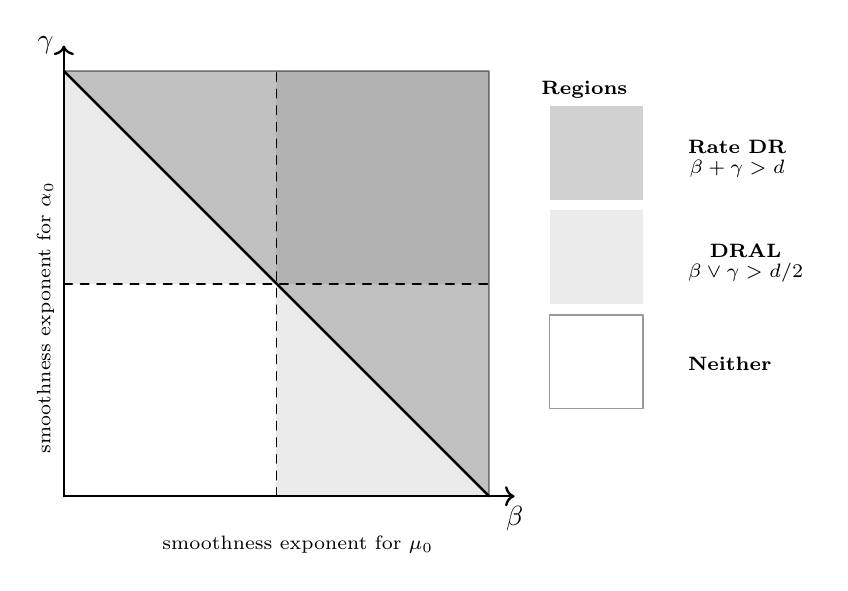
\begin{tikzpicture}[x=5.4cm,y=5.4cm, line cap=round, line join=round]
\def\half{0.5} % = d/2 when d=1

% --- Styles
\tikzset{
  regionDRAL/.style={fill=black, fill opacity=0.08, draw=none},
  regionPR/.style={fill=black, fill opacity=0.18, draw=none},
  boundary/.style={line width=0.85pt},
  guide/.style={dash pattern=on 3pt off 3pt, line width=0.65pt},
  axis/.style={->, line width=0.85pt},
}

% --- Frame
\draw[black!40, line width=0.55pt] (0,0) rectangle (1,1);

% --- Regions (CORRECT)
% DRAL: beta>=1/2 OR gamma>=1/2  (union of two rectangles)
\fill[regionDRAL] (\half,0) rectangle (1,1); % beta >= 1/2
\fill[regionDRAL] (0,\half) rectangle (1,1); % gamma >= 1/2

% Product-rate: beta+gamma>1 (triangle above diagonal), drawn on top
\fill[regionPR] (0,1) -- (1,0) -- (1,1) -- cycle;

% --- Boundaries
\draw[boundary] (0,1) -- (1,0);        % beta+gamma=1
\draw[guide] (\half,0) -- (\half,1);   % beta=1/2
\draw[guide] (0,\half) -- (1,\half);   % gamma=1/2

% --- Axes
\draw[axis] (0,0) -- (1.06,0) node[below] {$\beta$};
\draw[axis] (0,0) -- (0,1.06) node[left] {$\gamma$};

% Axis titles
\node[below] at (0.55,0) [yshift=-11pt] {\scriptsize smoothness exponent for $\mu_0$};
\node[rotate=90, anchor=south] at (0,0.55) [xshift=-20pt]
  {\scriptsize smoothness exponent for $\alpha_0$};
  
 
% --- Compact legend (heading centered over the *text* column)
\node[anchor=north west] at (1.10,1.00) {\scriptsize\textbf{Regions}};
\node[anchor=north west, align=left] at (1.10,0.94) {\scriptsize
\renewcommand{\arraystretch}{1.15}
\begin{tabular}{@{}c@{\qquad}l@{}}
% Rate DR row: heading centered above the formula
\begin{tabular}[c]{@{}c@{}}
\raisebox{1pt}{\tikz\fill[regionPR] (0,0) rectangle (0.22,0.22);}
\end{tabular}
&
\begin{tabular}[c]{@{}c@{}}
\textbf{Rate DR}\\[-2pt]
$\beta+\gamma>d$
\end{tabular}
\\[8pt]
% DRAL row: heading centered above the formula
\begin{tabular}[c]{@{}c@{}}
\raisebox{1pt}{\tikz\fill[regionDRAL] (0,0) rectangle (0.22,0.22);}
\end{tabular}
&
\begin{tabular}[c]{@{}c@{}}
\textbf{DRAL}\\[-2pt]
$\beta\vee\gamma>d/2$
\end{tabular}
\\[8pt]
\raisebox{1pt}{\tikz\draw[black!40, line width=0.55pt] (0,0) rectangle (0.22,0.22);}
&
\begin{tabular}[c]{@{}c@{}}
\textbf{Neither}\\[30pt]
\end{tabular}
\end{tabular}
};

\end{tikzpicture}
\caption{Smoothness trade-offs for asymptotic linearity. Under H\"older-type
rates \(n^{-\beta/(2\beta+d)}\) and \(n^{-\gamma/(2\gamma+d)}\), rate double
robustness typically requires \(\beta+\gamma>d\), whereas DRAL requires only
\(\beta\vee\gamma>d/2\).}
\label{fig:smoothness_tradeoff}
\end{figure}



To elucidate how doubly robust asymptotic linearity can arise, we study the
one-step debiased estimator \(\tau_n\) under possible nuisance
misspecification. Suppose that \(\alpha_n \to_p \overline{\alpha}_0\) and
\(\mu_n \to_p \overline{\mu}_0\) in the sense that
\(\|\alpha_n-\overline{\alpha}_0\|=o_p(1)\) and
\(\|\mu_n-\overline{\mu}_0\|=o_p(1)\), where at least one limit is correct,
i.e., either \(\overline{\mu}_0=\mu_0\) or \(\overline{\alpha}_0=\alpha_0\).
Under sample splitting, or under suitable estimator-complexity conditions, we
obtain a von Mises-type expansion \citep{benkeser2017doubly}
\begin{equation}
  \tau_n - \tau_0
  = (P_n - P_0)\,\overline{D}_0
    + o_p(n^{-1/2})
    + \langle \alpha_0 - \alpha_n, \mu_n - \mu_0 \rangle,
  \label{eqn::drbias2}
\end{equation}
where \(\overline{D}_0 := \phi_{0,\overline{\mu}_0}
+ D_{\overline{\mu}_0,\overline{\alpha}_0}\). Thus, up to the
\(o_p(n^{-1/2})\) term, the only obstruction to asymptotic linearity of
\(\tau_n\) is the cross-product remainder
\(\langle \alpha_0-\alpha_n,\,\mu_n-\mu_0\rangle\). Most of the existing
literature controls this remainder via rate double robustness, imposing the
product-rate condition \(\|\alpha_n-\alpha_0\|\,\|\mu_n-\mu_0\|=o_p(n^{-1/2})\),
which typically requires both nuisance estimators to be consistent and to
converge sufficiently fast \citep{robinsCausal,robins1995analysis,
vanderLaanRose2011,DoubleML}. If both limits are correct, so that
\(\overline{\mu}_0=\mu_0\) and \(\overline{\alpha}_0=\alpha_0\), then
\(\overline{D}_0\) coincides with the efficient influence function \(D_0\) in
Theorem~\ref{theorem::EIF}, yielding efficiency.




When the product-rate condition fails---because one nuisance estimator is
inconsistent or converges too slowly---the cross-product remainder in
\eqref{eqn::drbias2} is no longer negligible and can dominate
\(n^{1/2}(\tau_n-\tau_0)\), precluding asymptotic linearity of the one-step
estimator. Achieving DRAL therefore requires
additional control or debiasing of \(\langle \alpha_0-\alpha_n,\,\mu_n-\mu_0\rangle\)
so that it is negligible, or admits an asymptotically linear representation,
even without \(\|\alpha_n-\alpha_0\|\,\|\mu_n-\mu_0\|=o_p(n^{-1/2})\). In the
remainder of this section, we analyze this term and show how additional
debiasing yields DRAL whenever either (i) or (ii) holds, under suitable
conditions. Readers primarily interested in the estimator may wish to proceed
directly to Section~\ref{section::proposedestimator}.




 
 

\subsection{General strategy: debiasing the cross-product remainder}
\label{sec::genstrat}

\subsubsection{A learner-agnostic bias expansion under calibration and partial orthogonality}


We now describe a general strategy for debiasing the cross-product
remainder $\langle \alpha_0 - \alpha_n, \mu_n - \mu_0 \rangle$ by
further calibrating the nuisance estimators $\alpha_n$ and $\mu_n$.
The aim is to construct these estimators so that the cross-product
remainder admits an asymptotically linear representation, behaving like
the empirical mean of a mean-zero (possibly degenerate) influence
function. This strategy builds on approaches developed in
\cite{van2014targeted} and subsequent work
\citep{benkeser2017doubly, diaz2017doubly, diaz2019statistical, dukes2024doubly},
which construct DRAL estimators of average treatment effects in settings
where one nuisance estimator may be inconsistent. Here, we extend this line of work in two directions. First, we consider a
broad class of statistical parameters beyond the average treatment
effect. Second, we analyze regimes in which both nuisance estimators are
consistent but one may converge at an arbitrarily slow rate. In these settings, we
establish asymptotic linearity of the cross-product remainder and provide
refined conditions under which the remaining higher-order terms are
asymptotically negligible.


 
To formalize this strategy, define the nuisance estimation errors
\(\Delta_{\alpha,n} := \alpha_n - \alpha_0\) and
\(\Delta_{\mu,n} := \mu_n - \mu_0\), and let \(s_{n,0}\) and \(r_{n,0}\) denote
the projections of \(\alpha_0-\alpha_n\) and \(\mu_0-\mu_n\) onto functions of
\(\mu_n\) and \(\alpha_n\), respectively:
\[
s_{n,0} := \Pi_{\mu_n}(\alpha_0 - \alpha_n),
\qquad
r_{n,0} := \Pi_{\alpha_n}(\mu_0 - \mu_n).
\]
Here, for any feature map
$v \colon \mathcal{A} \times \mathcal{W} \to \mathbb{R}^k$, $k \in \mathbb{N}$,
the projection operator $\Pi_v \colon \mathcal{H} \to \mathcal{H}$ is defined as
\[
\Pi_v f := \arg\min_{\theta \in \Theta_v} \|f - \theta\|,
\qquad
\Theta_v := \{ h \circ v : h \colon \mathbb{R}^k \to \mathbb{R} \}.
\]
When $v$ and $f$ are nonrandom functions, the quantity
$(\Pi_v f)(a,w) = E_0\{f(A,W) \mid v(A,W) = v(a,w)\}$ coincides with the
conditional expectation of $f(A,W)$ given $v(A,W)$.


 


 
 
Our debiasing strategy calibrates the nuisance estimators to impose a minimal form of empirical orthogonality between their errors, thereby linearizing the cross-product remainder. Specifically, we construct calibrated nuisance estimators $\mu_n$ and $\alpha_n$ that satisfy the empirical orthogonality conditions
\begin{equation}
\frac{1}{n}\sum_{i=1}^n s_{n,0}(A_i,W_i)\{Y_i - \mu_n(A_i,W_i)\}
= 0 ,
\label{eqn::orthogonaloutcome}
\end{equation}
\begin{equation}
\psi_n(r_{n,0})
- \frac{1}{n}\sum_{i=1}^n r_{n,0}(A_i, W_i)\,\alpha_n(A_i, W_i)
= 0 .
\label{eqn::orthogonalRiesz}
\end{equation}
 The first condition makes the regression residuals $Y_i-\mu_n(A_i,W_i)$
empirically orthogonal to the component of the Riesz error
$\Delta_{\alpha,n}$ explained by one-dimensional functions of $\mu_n$.
The second enforces the empirical Riesz representation
$\psi_n(r_{n,0})=\langle \alpha_n, r_{n,0}\rangle_{P_n}$ along directions
corresponding to the component of the regression error $\Delta_{\mu,n}$
explained by one-dimensional functions of $\alpha_n$. When
$\psi_n(\cdot)=\langle \cdot\,, \alpha_n^\star\rangle_{P_n}$ for some
empirical representer $\alpha_n^\star\in L^2(P_n)$, this condition is equivalent to
$\langle r_{n,0},\alpha_n^\star-\alpha_n\rangle_{P_n}=0$. For the average treatment effect, \cite{benkeser2017doubly}
approximately satisfied these conditions using parameter-specific
TMLE-style procedures (see Appendix~\ref{sec::drtmle}) based on estimates
of $r_{n,0}$ and $s_{n,0}$. In the next section we present a simple approach for
constructing such estimators using isotonic calibration. Here we explain how
these conditions arise and why they suffice to debias the cross-product remainder. For now, we assume that nuisance estimators $\mu_n$ and $\alpha_n$ satisfying \eqref{eqn::orthogonaloutcome} and \eqref{eqn::orthogonalRiesz} are available.



 

 

To build intuition, we first study the cross-product remainder under \eqref{eqn::orthogonaloutcome} and show how this condition reduces sensitivity to estimation error in \(\alpha_n\) when \(\mu_n\) is consistent for \(\mu_0\). Following \cite{van2014targeted} and related work, we begin with the observation that the cross-product remainder depends only on the component of the Riesz estimation error \(\alpha_n(A,W)-\alpha_0(A,W)\) lying in the linear span of \(\mu_n(A,W)\) and \(\mu_0(A,W)\). Specifically, by the law of iterated expectations, conditioning on \((\mu_n(A,W),\mu_0(A,W))\) under \(P_0\) yields
\begin{align*}
\langle \alpha_0 - \alpha_n , \mu_n - \mu_0 \rangle
&= \langle \Pi_{(\mu_n, \mu_0)}(\alpha_0 - \alpha_n), \mu_n - \mu_0\rangle.
\end{align*}
The orthogonality condition \eqref{eqn::orthogonaloutcome} then applies a minimal correction to the identifiable component \(\Pi_{\mu_n}(\alpha_0-\alpha_n)\) of the projected error \(\Pi_{(\mu_n,\mu_0)}(\alpha_0-\alpha_n)\), that is, the part determined by \(\mu_n(A,W)\). Specifically, following \cite{benkeser2017doubly}, \cite{dukes2024doubly}, and \cite{bonvini2024doubly}, we decompose the preceding display as
\begin{equation}
\label{eqn::DRexpansion}
\begin{aligned}
\langle \alpha_0 - \alpha_n , \mu_n - \mu_0 \rangle
&= \langle \Pi_{\mu_n}(\alpha_0 - \alpha_n), \mu_n - \mu_0\rangle
  + \langle (\Pi_{(\mu_n , \mu_0)} - \Pi_{\mu_n})(\alpha_0 - \alpha_n),
           \mu_n - \mu_0\rangle \\
&= \langle s_{n,0}, \mu_n - \mu_0\rangle
  - \langle (\Pi_{(\mu_n , \mu_0)} - \Pi_{\mu_n}) \Delta_{\alpha,n},
           \mu_0 - \Pi_{\mu_n} \mu_0 \rangle,
\end{aligned}
\end{equation}
where the second term is negligible when \(\mu_0\) provides little information about the residual \(\Delta_{\alpha,n}\) beyond what is already captured by \(\mu_n\). The first term is the leading bias component and can prevent asymptotic linearity of \(\tau_n\) when \(\alpha_0\) is estimated too slowly or inconsistently. The key role of \eqref{eqn::orthogonaloutcome} is to convert this leading term into an empirical process fluctuation:
\[
\langle s_{n,0}, \mu_n - \mu_0\rangle
= - P_0 A_{n,0}
= (P_n - P_0) A_{n,0}
= (P_n-P_0) A_0 + (P_n - P_0) (A_{n,0} - A_0),
\]
where \(A_{n,0}(z) := s_{n,0}(a,w)\{y - \mu_n(a,w)\}\), \(A_0(z) := s_0(a,w)\{y - \mu_0(a,w)\}\), \(s_0 := \Pi_{\mu_0}(\alpha_0 - \overline{\alpha}_0)\), and the second equality uses \(P_n A_{n,0}=0\) from \eqref{eqn::orthogonaloutcome}. Provided that \(\|A_{n,0}-A_0\|=o_p(1)\) and \(A_{n,0}\) satisfies an appropriate empirical process condition, the final term on the right is \(o_p(n^{-1/2})\); we verify this condition for isotonic calibration in our proofs.

% , we can typically show \((P_n-P_0)A_{n,0}=(P_n-P_0)A_0+o_p(n^{-1/2})\),
% so this term is asymptotically linear, or negligible when \(A_0=0\) (e.g.,
% when \(\overline{\alpha}_0=\alpha_0\)).   

 

 


   



 % Importantly, the second term is typically smaller than the original cross-product
%remainder because it replaces $\Delta_{\alpha,n}$ and $\Delta_{\mu,n}$ with the
%residuals $\Pi_{(\mu_n , \mu_0)}\Delta_{\alpha,n}-\Pi_{\mu_n}\Delta_{\alpha,n}$ and$\Delta_{\mu,n}-\Pi_{\mu_n}\Delta_{\mu,n}$, %removing the components of the
%nuisance estimation errors explained by $\mu_n$. The second term in
%\eqref{eqn::DRexpansion} is a higher-order remainder that is negligible under
%our conditions.  


 


The following theorem formalizes the above by deriving a bias expansion showing
how \eqref{eqn::orthogonaloutcome} and \eqref{eqn::orthogonalRiesz} debias the
cross-product remainder. To control the higher-order terms in
\eqref{eqn::DRexpansion} and related expansions, we impose the following
high-level condition, with sufficient conditions given later. Informally, we
require that the estimation error of the slower or inconsistent nuisance be
asymptotically orthogonal after partialling out the other nuisance:
\begin{enumerate}[label=\bf{B\arabic*)}, ref={B\arabic*},series=sketch]
  \item \textit{Asymptotic partial orthogonality:} At least one of the following holds: \label{cond:ortho} 
    \begin{enumerate}[label={\roman*)}, ref={\ref{cond:ortho}\roman*}]\vspace{-.05in}
      \item \label{cond:orthoA} \(\langle (\Pi_{(\mu_n , \mu_0)}-\Pi_{\mu_n})\Delta_{\alpha,n}
        \,,\, \mu_0 - \Pi_{\mu_n} \mu_0 \rangle = O_p(\|\mu_n -  \mu_0\|^2)\),\vspace{-.05in}
      \item \label{cond:orthoB} \(\langle (\Pi_{(\alpha_n , \alpha_0)}-\Pi_{\alpha_n})\Delta_{\mu,n}
        \,,\, \alpha_0 - \Pi_{\alpha_n} \alpha_0 \rangle = O_p(\|\alpha_n -  \alpha_0\|^2)\).
    \end{enumerate}
\end{enumerate}
The term in \ref{cond:orthoA} is a covariance between the
component of \(\Pi_{(\mu_n,\mu_0)}\Delta_{\alpha,n}\) that remains after
partialling out functions of \(\mu_n\) and the approximation error
\(\mu_0-\Pi_{\mu_n}\mu_0\). When this condition holds, the higher-order term in
\eqref{eqn::DRexpansion} is \(O_p(\|\mu_n-\mu_0\|^2)\), and is therefore
asymptotically negligible when \(\|\mu_n-\mu_0\| = o_P(n^{-1/4})\), regardless
of the quality of \(\alpha_n\). Similarly, Condition~\ref{cond:orthoB} ensures a related higher-order term is negligible  with the roles of $\alpha$ and $\mu$ reversed. We provide sufficient conditions in Section \ref{sec::sufficientconds}. As a concrete example, Condition~\ref{cond:orthoA} holds if \(\Pi_{(\mu_n,\mu_0)}\Delta_{\alpha,n}\) admits the approximate partially linear representation 
\begin{equation}
\label{eqn::PLM}
    \Pi_{(\mu_n,\mu_0)}\Delta_{\alpha,n} = g_n \circ \mu_n + \beta_n \circ (\mu_n,\mu_0)\cdot(\mu_n-\mu_0) + o_p(\|\mu_n-\mu_0\|)
\end{equation}
in \(L^2(P_0)\), for some \(g_n\colon \mathbb{R}\to\mathbb{R}\) and \(\beta_n\colon \mathbb{R}^2\to\mathbb{R}\) satisfying \(\|\beta_n\|_{\infty}=O_p(1)\). In particular, this condition holds if \((\Pi_{(\mu_n,\mu_0)}\Delta_{\alpha,n})(A,W)\) is sufficiently smooth in \(\mu_n(A,W)\) and \(\mu_0(A,W)\).

 



In the following theorem, we also define
$r_0 := \Pi_{\alpha_0}(\mu_0 - \overline{\mu}_0)$, 
$B_0 := \phi_{r_0} +  \psi_0(r_0)  - r_0 \alpha_0$, and
$B_{n,0} :=\phi_{r_{n,0}} +  \psi_0(r_{n,0})  - r_{n,0} \alpha_n$.
The theorem does not require the nuisance estimators $\mu_n$ and $\alpha_n$
to converge to $\overline{\mu}_0$ and $\overline{\alpha}_0$, but we assume
this convergence in all subsequent results and in the discussion that follows.




 
  
\begin{theorem}[Expansion of cross-product remainder under orthogonality]
\label{theorem::DRbiasexpansion} Both of the following are valid:
\begin{enumerate}[label=(\roman*)]
    \item \emph{Regression-based decomposition:} If $\mu_n$ satisfies \eqref{eqn::orthogonaloutcome}, 
\begin{align*}
\langle \alpha_0 - \alpha_n, \mu_n - \mu_0 \rangle  &= P_n A_0 +  (P_n - P_0)(A_{n,0} - A_0)  + \langle (\Pi_{(\mu_n, \mu_0)} - \Pi_{\mu_n})\Delta_{\alpha,n}, \,\mu_0 - \Pi_{\mu_n} \mu_0 \rangle
\end{align*}
 If \ref{cond:orthoA} holds, then
$ \langle (\Pi_{(\mu_n, \mu_0)} - \Pi_{\mu_n})\Delta_{\alpha,n}, \,\mu_0 - \Pi_{\mu_n} \mu_0 \rangle
= O_p\left(\|\mu_n - \mu_0 \|^2\wedge\|\Pi_{\mu_n}\mu_0 - \mu_0 \|\|\alpha_n - \alpha_0\| \right)$. 
\item \emph{Riesz-representer-based decomposition:} If $\alpha_n$ satisfies \eqref{eqn::orthogonalRiesz}, 
\begin{align*}
\langle \alpha_0 - \alpha_n, \mu_n - \mu_0 \rangle  &=  P_n B_0 +  (P_n - P_0)(B_{n,0} - B_0) + \langle (\Pi_{(\alpha_n, \alpha_0)} + \Pi_{\alpha_n})\Delta_{\mu,n}, \,\alpha_0 - \Pi_{\alpha_n} \alpha_0 \rangle   + Rem_{\psi_n}(r_{n,0}),
\end{align*}
 with
$ Rem_{\psi_n}(r_{n,0}) := \psi_n(r_{n,0}) - \psi_0(r_{n,0}) - P_n \phi_{r_{n,0}}$. If \ref{cond:orthoB} holds, then
$\langle (\Pi_{(\alpha_n, \alpha_0)} - \Pi_{\alpha_n})\Delta_{\mu,n}, \,\Delta_{\alpha,n} \rangle
=  O_p\left(\|\alpha_n - \alpha_0 \|^2 \wedge\|\mu_n - \mu_0 \|\|\Pi_{\alpha_n}\alpha_0 - \alpha_0\| \right)$.
 
\end{enumerate}

 

 
 
\end{theorem}
When the nuisance estimators satisfy the empirical orthogonality conditions in \eqref{eqn::orthogonaloutcome} and \eqref{eqn::orthogonalRiesz}, Theorem~\ref{theorem::DRbiasexpansion} decomposes the cross-product remainder into an asymptotically linear term, an empirical-process remainder, and a higher-order cross-product remainder. Under the regression-based decomposition, these terms are \(P_nA_0\), \((P_n-P_0)(A_{n,0}-A_0)\), and \(\langle (\Pi_{(\mu_n,\mu_0)}-\Pi_{\mu_n})\Delta_{\alpha,n},\, \mu_0-\Pi_{\mu_n}\mu_0\rangle\).  Recalling \eqref{eqn::drbias2}, if the remainder terms are \(o_p(n^{-1/2})\), then the one-step debiased estimator \(\tau_n\), constructed from the orthogonalized nuisance estimators \(\mu_n\) and \(\alpha_n\), is DRAL with influence function \(\overline{D}_0 + 1(\overline{\mu}_0 \neq \mu_0)\,A_0 + 1(\overline{\alpha}_0 \neq \alpha_0)\,B_0\).  Moreover, if both nuisance estimators are consistent, so that \(\overline{\alpha}_0=\alpha_0\) and \(\overline{\mu}_0=\mu_0\), then \(A_0=0\) and \(B_0=0\). Hence, \(\tau_n\) is asymptotically linear with influence function \(\overline{D}_0\), provided the cross-product remainder is purely second order.


 


The higher-order cross-product remainder can be bounded using the Cauchy--Schwarz inequality. This is the same approach typically used to bound the traditional cross-product remainder, for which it yields $|\langle \alpha_0 - \alpha_n, \mu_n - \mu_0 \rangle|
\le \|\alpha_n-\alpha_0\|\,\|\mu_n - \mu_0\|$
\citep{vanderLaanRose2011, chernozhukov2018double, bonvini2024doubly}. For the higher-order cross-product remainder, Cauchy--Schwarz yields
\begin{equation}
 \big|
 \langle (\Pi_{(\mu_n, \mu_0)} - \Pi_{\mu_n})\Delta_{\alpha,n},
  \,\mu_0 - \Pi_{\mu_n} \mu_0 \rangle
 \big|
 \leq
 \| (\Pi_{(\mu_n, \mu_0)} - \Pi_{\mu_n})(\alpha_n - \alpha_0)\|\,
 \|\mu_0 - \Pi_{\mu_n} \mu_0\|.
 \label{eqn::worstcasebound}
\end{equation}
This bound is tighter than the bound on \(|\langle \alpha_0 - \alpha_n, \mu_n - \mu_0 \rangle|\) because it projects out the components of the nuisance errors explained by \(\mu_n\). Under \ref{cond:orthoA}, this dominance is even clearer, since then \eqref{eqn::worstcasebound} converges to $0$ at least as quickly as the faster of $\|\mu_n - \mu_0 \|^2$ and $\|\alpha_n - \alpha_0\|\|\Pi_{\mu_n}\mu_0 - \mu_0 \|=O_p(\|\alpha_n-\alpha_0\|\|\mu_n - \mu_0\|)$. Analogous bounds hold for the Riesz-based decomposition, in which \(\alpha_n\) is projected out from both errors.

 

 

%\subsubsection{Sufficient conditions for partial orthogonality.}
%\label{sec::sufficientconds}

%{\color{red}The partial orthogonality conditions in \ref{cond:ortho} are high-level and
%minimal but, \emph{a priori}, are not obviously satisfied in practice.} {\color{blue}A
%pathological counterexample  for \ref{cond:orthoA} arises when the projected regression error is exactly aligned
%with the Riesz error, that is, \(\mu_0 - \Pi_{\mu_n} \mu_0  = \varepsilon_n \Delta_{\alpha,n} / \|\Delta_{\alpha,n}\|\) for some $\varepsilon_n=o(1)$. In this case,
%\(\langle (\Pi_{(\mu_n , \mu_0)}-\Pi_{\mu_n})\Delta_{\alpha,n}
%        \,,\, \mu_0 - \Pi_{\mu_n} \mu_0 \rangle = 
%\|\Delta_{\alpha,n}\| \|\mu_0-\Pi_{\mu_n}\mu_0\|\) may converges slower than $\|\mu_n - \mu_0\|^2$, especially when $\|\Delta_{\alpha,n}\|$ does not converge to $0$ in probability.} Nonetheless, this and other counterexamples are ruled out by existing conditions in the literature ({\color{red} Condition (v) in Appendix F of \cite{benkeser2020nonparametric}; Theorem 1 of \cite{benkeser2017doubly}; Assumption 3  of \cite{dukes2024doubly}; Lemma I.1 of \cite{wang2023super}; and Section 3.1 of \cite{bonvini2024doubly}}). We adapt these conditions to our setting and present them in order of increasing strength.  


%By contrast, as discussed in the previous section, this condition holds if \(\Pi_{(\mu_n,\mu_0)}\Delta_{\alpha,n} = g_n \circ \mu_n + \beta_n \circ (\mu_n,\mu_0)\cdot(\mu_n-\mu_0) + o_p(\|\mu_n-\mu_0\|)\) in \(L^2(P_0)\). In particular, in the misspecified case, it holds if \(\overline{\alpha}_0(A,W) - \alpha_0(A,W) = g_0(\mu_0(A,W))\), where \(g_0\) is continuously differentiable, and \(\|\alpha_n - \overline{\alpha}_0\| = O_p(\|\mu_n - \mu_0\|)\).


 
\subsubsection{Sufficient conditions for partial orthogonality}
\label{sec::sufficientconds}

% The partial orthogonality requirements in \ref{cond:ortho} are high-level geometric conditions. One
A sufficient condition for \ref{cond:ortho} is that the projected Riesz error \(\Pi_{(\mu_n,\mu_0)}\Delta_{\alpha,n}\) admits the partially linear expansion in \eqref{eqn::PLM}. At a high level, \ref{cond:orthoA} rules out near-perfect alignment between the projected-out regression error and the Riesz error. For example, if \(\mu_0 - \Pi_{\mu_n}\mu_0 = \varepsilon_n \Delta_{\alpha,n}/\|\Delta_{\alpha,n}\|\) for some \(\varepsilon_n=o(1)\), then \(\langle (\Pi_{(\mu_n,\mu_0)}-\Pi_{\mu_n})\Delta_{\alpha,n}, \mu_0-\Pi_{\mu_n}\mu_0\rangle\) is of order \(\|\Delta_{\alpha,n}\|\,\|\mu_0-\Pi_{\mu_n}\mu_0\|\), which need not be \(o_p(\|\mu_n-\mu_0\|^2)\), especially when \(\|\Delta_{\alpha,n}\|\) does not converge to zero in probability. Conditions excluding this type of behavior already appear in related work; see, for example, Condition~(v) in Appendix~F of \citet{benkeser2020nonparametric}, Theorem~1 of \citet{benkeser2017doubly}, Assumption~3 of \citet{dukes2024doubly}, Lemma~I.1 of \citet{wang2023super}, and Section~3.1 of \citet{bonvini2024doubly}. We next adapt these ideas to our setting and present sufficient conditions in increasing order of strength.

 

 %Suppose $\overline{\alpha}_0(A,W) - \alpha_0(A,W) = g_0(\mu_0(A,W))$ with $g_0 \in C^1$. Then, a pointwise Taylor expansion gives: $\overline{\alpha}_0 - \alpha_0  = g_0 \circ \mu_n + (g_0' \circ \mu_n) (\mu_n - \mu_0) + o(\|\mu_n - \mu_0\|)$. Hence, by the triangle inequality, $\Pi_{(\mu_n,\mu_0)}\Delta_{\alpha,n}
%= g_n\circ\mu_n+\beta_n \circ (\mu_n,\mu_0) (\mu_n-\mu_0) + O_p(\|\mu_n-\mu_0\|)$ provided that $\Pi_{\mu_n, \mu_0}(\alpha_n - \overline{\alpha}_0) =  \widetilde{g}_{n} \circ \mu_n + O_p(\|\mu_n-\mu_0\|)$ for some $\widetilde{g}_{n}$ and \ref{cond:orthoA} holds.


 



  \begin{enumerate}[label=\bf{\ref{cond:ortho}$^{*}$}, ref={\ref{cond:ortho}$^{*}$}]
  \item \textit{Projection error coupling}  \citep{van2014targeted}: \label{cond:projectioncoupling1}  
      \begin{enumerate}[label={\roman*)}, ref={\ref{cond:projectioncoupling1}\roman*}]\vspace{-.05in}
     \item \label{cond:projectioncoupling1A}   $  \|(\Pi_{\mu_n, \mu_0} - \Pi_{\mu_n})\Delta_{\alpha,n}\|  =   O_p(\|\mu_n - \mu_0 \|)$\,; \vspace{-.05in}
     \item \label{cond:projectioncoupling1B}   $\|(\Pi_{\alpha_n, \alpha_0} - \Pi_{\alpha_n})\Delta_{\mu,n}\|  = O_p( \|\alpha_n - \alpha_0 \|)$\,.
 
    \end{enumerate}

\end{enumerate}
The above condition is also assumed in \citet[][Theorem~1]{benkeser2017doubly} and \citet[][Assumption~3]{dukes2024doubly}; related conditions appear in \cite{diaz2017doubly} and \cite{diaz2019statistical}.
  \begin{enumerate}[label=\bf{\ref{cond:ortho}$^{**}$}, ref={\ref{cond:ortho}$^{**}$}]
    \item\textit{Lipschitz continuity} 
\citep{bonvini2024doubly}: Denoting\ $\mathcal{D}_n := \{Z_1,\ldots,Z_n\}$, it holds that, for all $n$ large enough:\label{cond:projectioncoupling2}  
    \begin{enumerate}[
  label={\roman*)},
  ref=\ref{cond:projectioncoupling2}\roman*,
  leftmargin=-10pt,
  labelsep=-0.7em,
  labelindent=0pt,
  align=left
]\item $(\widehat{m}, m) \mapsto E_0\{\Delta_{\alpha,n}(A,W) \,|\,  \mu_n(A,W) = \widehat{m}, \mu_0(A,W) = m, \mathcal{D}_n\}$ is $P_0$--almost surely Lipschitz continuous with uniformly bounded constant;\label{cond:projectioncoupling2A}  
    \item  $(\widehat{a}, a) \mapsto E_0\{\Delta_{\mu,n}(A,W) \,|\,  \alpha_n(A,W) = \widehat{a}, \alpha_0(A,W) = a, \mathcal{D}_n\}$ is $P_0$--almost surely Lipschitz continuous with uniformly bounded constant.\label{cond:projectioncoupling2B}  
    \end{enumerate}
    
\end{enumerate}
The above condition is also used in \citet[][Section~3.1]{bonvini2024doubly} and related bounded derivative conditions were also imposed in \citet[][Condition~v in Appendix~F]{benkeser2020nonparametric}, \citet[][Lemma~1]{van2023adaptive}, and \citet[][Lemma~I.1]{wang2023super} to analyze regressions involving estimated features.


 \begin{lemma}[Sufficient conditions for \ref{cond:ortho}]
 \label{lemma::sufficientcoupling}
Conditions \ref{cond:orthoA} and \ref{cond:orthoB} are implied by
\ref{cond:projectioncoupling1A} and \ref{cond:projectioncoupling1B},
respectively. Moreover, \ref{cond:projectioncoupling1A} and
\ref{cond:projectioncoupling1B} are implied by
\ref{cond:projectioncoupling2A} and \ref{cond:projectioncoupling2B},
respectively.
\end{lemma}
 
 

Roughly, Condition~\ref{cond:projectioncoupling1A} requires that \(\Pi_{(\mu_n,\mu_0)}\Delta_{\alpha,n}\) be well approximated by \(\Pi_{\mu_n}\Delta_{\alpha,n}\) whenever \(\mu_n\) converges to \(\mu_0\) in norm. Heuristically, it asserts that, as \(\|\mu_n-\mu_0\|\to 0\), the information in \(\{\mu_n(A,W),\mu_0(A,W),Z_1,\ldots,Z_n\}\) for predicting \(\Delta_{\alpha,n}\) is asymptotically equivalent to that in \(\{\mu_n(A,W),Z_1,\ldots,Z_n\}\). While such equivalences need not hold in general, a sufficient condition is Condition~\ref{cond:projectioncoupling2}, which ensures that \(\Pi_{(\mu_n,\mu_0)}\Delta_{\alpha,n}\) and \(\Pi_{(\alpha_n,\alpha_0)}\Delta_{\mu,n}\) are almost surely Lipschitz continuous as bivariate transformations of \((\mu_n,\mu_0)\) and \((\alpha_n,\alpha_0)\), respectively. By symmetry between \(\mu_n\) and \(\mu_0\), Condition~\ref{cond:projectioncoupling2A} also implies \(\|(\Pi_{(\mu_n,\mu_0)}-\Pi_{\mu_0})\Delta_{\alpha,n}\| = O_p(\|\mu_n-\mu_0\|)\) and hence, by the triangle inequality, \(\|(\Pi_{\mu_0}-\Pi_{\mu_n})\Delta_{\alpha,n}\| = O_p(\|\mu_n-\mu_0\|)\). An analogous conclusion holds for Condition~\ref{cond:projectioncoupling2B}. Conditions~\ref{cond:ortho}--\ref{cond:projectioncoupling2} can also be relaxed to H\"older-type continuity \citep{bonvini2024doubly}; in that case, a weaker form of the bias expansion in Theorem~\ref{theorem::DRbiasexpansion}, governed by the H\"older exponent, can still be established.

More broadly, some form of structural assumption is unavoidable for
meaningfully improving upon standard doubly robust estimators, since
first-order methods are optimal in structure-agnostic settings
\citep{balakrishnan2023fundamental, jin2025sharp}. Conditions
\ref{cond:ortho}--\ref{cond:projectioncoupling2} provide one such set of
assumptions. For comparison, analyses of higher-order influence function
estimators \citep{robins2008higher} typically impose H\"older-type smoothness
assumptions on the potentially high-dimensional error functions
\(\Delta_{\mu,n}\) and \(\Delta_{\alpha,n}\), whereas sparsity-based methods
require approximate sparsity and linearity of the nuisance models
\citep{liu2023root}. Our guarantees instead rely on the \emph{asymptotic
partial orthogonality} condition in \ref{cond:ortho}, which is qualitatively
different from the smoothness and approximability assumptions used in these
approaches. In particular, the sufficient Condition~\ref{cond:projectioncoupling2}
requires only smoothness of certain bivariate transformations of the true and
estimated nuisances. Informally, Condition~\ref{cond:projectioncoupling2A} may be
plausible when the joint level sets
\(\{(a,w): \mu_n(a,w)=\widehat m,\ \mu_0(a,w)=m\}\) vary smoothly with
\((\widehat m,m)\), and the conditional mean of \(\Delta_{\alpha,n}\) over
these level sets depends continuously on \((\widehat m,m)\). Finally,  \eqref{eqn::worstcasebound} shows that, even when these additional
conditions do not hold, the orthogonality conditions typically still attenuate
the bias of the one-step debiased estimator.
 
  

%Related questions about the stability of level sets under
%perturbations have been studied in differential geometry and topology, notably
%in Morse theory \citep{milnor1963morse, matsumoto2002introduction}, which may
%offer a useful lens for assessing such assumptions. 


%\paragraph{Relation to sparsity-based doubly robust inference via high-dimensional $\ell_1$-regularization.}
%Finally, our orthogonality-based approach to doubly robust inference is closely related to the (approximate) sparsity-based doubly robust literature discussed in the Introduction. When nuisances are estimated via $\ell_1$-regularized empirical risk minimization over linear classes, the Karush--Kuhn--Tucker (KKT) conditions imply approximate empirical orthogonality over suitable linear subspaces (see, e.g., \citealp[Eq.~15]{tan2020model}; \citealp[Sec.~2.1]{bradic2019sparsity}; \citealp[Sec.~4.1]{smucler2019unifying}). Under additional approximation conditions---typically requiring at least one nuisance error to be sufficiently sparse---this yields doubly robust asymptotic linearity for $\ell_1$-regularized autoDML estimators. \cite{liu2023root} show that this type of $\ell_1$-regularized, high-dimensional correction can be applied post hoc to initial $\ell_1$-regularized learners. For the outcome regression, their post-hoc correction can be viewed as enforcing a high-dimensional orthogonality objective---often called \emph{multi-accuracy} \citep{kim2019multiaccuracy, deng2023happymap, roth2022uncertain}---by targeting the moment conditions $E_{0}\left[(Y-\mu_n(A,W))\,f(A,W)\right]=0$ for all $f$ in a rich class (in their case, the span of the $\ell_1$ design/basis functions). For efficiency, this class must approximate the true representer $\alpha_0$ sufficiently well, so that $E_{0}\left[(Y-\mu_n(A,W))\,\alpha_0(A,W)\right]\approx 0$ (see Remark~3 in \cite{liu2023root}). In contrast, in Section~\ref{sec::genstrat}, we argue that it suffices to target a single moment condition, namely $E_{0}\left[(Y-\mu_n(A,W))\,s_{n,0}(A,W)\right]=0$, as in \eqref{eqn::orthogonaloutcome}. One can approximately enforce this condition via a TML-style update based on an estimate $\hat s_{n,0}$, as in \cite{benkeser2017doubly} and related work. Our approach, calibrated DML (Section~\ref{section::calibration}), instead targets the one-dimensional calibration constraint $\mu_n(A,W)=E_0\left[Y \mid \mu_n(A,W)\right]$, or, equivalently, the one-dimensional orthogonality conditions $E_{0}\left[(Y-\mu_n(A,W))\,\theta\bigl(\mu_n(A,W)\bigr)\right]=0$ for all $\theta:\mathbb{R}\to\mathbb{R}$.


 
 

\section{Calibrated debiased machine learning}
\label{section::proposedestimator}

\subsection{Enforcing orthogonality via calibration}
\label{section::calibration}


We now establish a key insight of this paper: the
empirical orthogonality equations \(\eqref{eqn::orthogonaloutcome}\) and
\(\eqref{eqn::orthogonalRiesz}\) can be enforced by calibrating the nuisance
estimators \(\mu_n\) and \(\alpha_n\).  Combined with Theorem~\ref{theorem::DRbiasexpansion} of the previous subsection, this
reformulation shows that calibration enables the construction of DRAL debiased
machine learning estimators, provided the nuisance estimators satisfy the
partial orthogonality conditions in \ref{cond:ortho}. In particular,
calibration implicitly performs the bias correction needed for the error
decomposition in Theorem~\ref{theorem::DRbiasexpansion} to apply. We now
formalize this connection and introduce our calibrated debiased machine
learning framework.





Calibration is a widely used post-hoc technique in predictive modeling that
transforms a model's fitted values to better align with the target they are
intended to predict \citep{lichtenstein1977calibration, zadrozny2002transforming,
niculescu2005predicting, bella2010calibration, guo2017calibration,
gupta2020distribution}. Motivated by this idea, we say that \(\mu_n\) and \(\alpha_n\) are
\emph{(perfectly) empirically calibrated} with respect to the least-squares and
Riesz losses if
\begin{align}
\sum_{i=1}^n \{Y_i - \mu_n(A_i, W_i)\}^2
&= \min_{\theta}\sum_{i=1}^n \{Y_i - \theta(\mu_n(A_i, W_i))\}^2,
\label{eqn::calpropertyoutcome} \\
\sum_{i=1}^n \{\alpha_n(A_i, W_i)\}^2 - 2 \psi_n(\alpha_n)
&= \min_{\theta}\Bigg\{
    \sum_{i=1}^n \{\theta(\alpha_n(A_i, W_i))\}^2
    - 2 \psi_n(\theta \circ \alpha_n)
  \Bigg\},
\label{eqn::calpropertyRiesz}
\end{align}
where the minima are taken over all one-dimensional functions
\(\theta:\mathbb{R}\to\mathbb{R}\). Equivalently, the empirical risk of each nuisance estimator cannot be reduced by
post-composing it with an arbitrary one-dimensional mapping
\citep{whitehouse2024orthogonal}.  Beyond enabling doubly robust inference, empirical calibration can improve
estimator stability and predictive accuracy. Calibration for the outcome regression ensures that $\mu_n(a,w)$ equals the empirical mean outcome
among individuals with the same predicted value, whereas calibration for the propensity
score enforces covariate balance across strata of the estimated propensity score
\citep{deshpande2023calibrated,van_der_Laan2024stabilized}.


 



 
Empirical calibration of the nuisance estimators implies the orthogonality
conditions \eqref{eqn::orthogonaloutcome} and \eqref{eqn::orthogonalRiesz}. To
ensure that this implication holds for \(\alpha_n\), we assume that the
estimated functional \(\psi_n\) is linear, as holds automatically for
\(\psi_n(\mu) := \frac{1}{n}\sum_{i=1}^n m(Z_i,\mu)\) in
Example~\ref{example::expectfunctional}.
\begin{enumerate}[label=\bf{B\arabic*)}, ref={B\arabic*},resume=sketch]
 \item \textit{(Linearity of the estimated functional)}
 \label{cond::estboundedlinear}
 \(P_0\)--almost surely, $\psi_n:\mathcal{H} \rightarrow \mathbb{R}$ satisfies \(\psi_n(c\mu_1 + \mu_2) = c\,\psi_n(\mu_1) + \psi_n(\mu_2)\)
 for each \(\mu_1,\mu_2\in \mathcal{H}\) and \(c\in\mathbb{R}\).
\end{enumerate}
 Under \ref{cond::estboundedlinear}, the first-order optimality conditions for
\eqref{eqn::calpropertyoutcome} and \eqref{eqn::calpropertyRiesz} yield the
equivalent moment conditions: for each transformation
\(\theta:\mathbb{R}\to\mathbb{R}\),
\begin{align}
    \frac{1}{n}\sum_{i=1}^n \theta\left(\mu_n(A_i,W_i)\right)\{Y_i - \mu_n(A_i,W_i)\}
    &= 0, \label{eqn::calpropertyoutcome2}\\
    \frac{1}{n}\sum_{i=1}^n \theta\left(\alpha_n(A_i,W_i)\right)\alpha_n(A_i,W_i)
    - \psi_n(\theta \circ \alpha_n)
    &= 0. \label{eqn::calpropertyRiesz2}
\end{align}
That is, calibration requires the residuals of \(\mu_n\) and \(\alpha_n\) to be
orthogonal to \emph{every} one-dimensional transformation of the corresponding
fitted values. In particular, they are orthogonal to the specific
transformations \(s_{n,0}=\Pi_{\mu_n}(\alpha_0 - \alpha_n)\) and
\(r_{n,0}=\Pi_{\alpha_n}(\mu_0 - \mu_n)\) appearing in the orthogonality conditions. We summarize this implication in the
following lemma.


\begin{lemma}[Empirical calibration debiases the cross-product remainder]
\label{theorem:empiricalcalibration}
If $\mu_n$ is empirically calibrated so that \eqref{eqn::calpropertyoutcome}
holds, then $\mu_n$ satisfies \eqref{eqn::orthogonaloutcome}. If, in addition, \ref{cond::estboundedlinear} holds and $\alpha_n$ satisfies
\eqref{eqn::calpropertyRiesz}, then $\alpha_n$ satisfies
\eqref{eqn::orthogonalRiesz}.
\end{lemma}
\noindent We refer to debiased machine learning with calibrated nuisance estimators as
\emph{calibrated DML}. 

In practice, calibration is implemented by applying a post-hoc one-dimensional map to an
initial nuisance estimator, chosen to reduce the empirical loss over a flexible class \citep{whitehouse2024orthogonal}.
A simple option is histogram (binning) calibration: partition the fitted values and assign a constant calibrated prediction within each bin, chosen to minimize the loss within that bin (e.g., an
empirical mean) \citep{zadrozny2001obtaining,gupta2021distribution,van2025generalized}.
A widely used alternative is \emph{isotonic calibration} \citep{zadrozny2002transforming,niculescu2005predicting},
which fits a monotone map and can be viewed as adaptive binning regularized by a
monotonicity constraint \citep{van2023causal,van2025generalized}. It is tuning-free and, unlike histogram binning, can only improve or leave unchanged the empirical risk, since the identity map is monotone. Moreover, the calibration properties in \eqref{eqn::calpropertyoutcome} and \eqref{eqn::calpropertyRiesz} follow from a basic property of isotonic regression: it yields a piecewise-constant fit, equivalently a histogram-binning estimator on a data-dependent partition of the input values produced by the pooled adjacent violators algorithm \citep{barlow1972isotonic}.
 

 
 


%The DRAL properties that arise from the calibration conditions in Lemma \ref{theorem:empiricalcalibration} relate to the fact that adjustment for either $\mu_0(A, W)$ or $\alpha_0(A, W)$ is sufficient for confounding bias adjustment. Notably, when $\psi_0$ is a counterfactual mean, adjusting for $\alpha_0(A, W)$ is equivalent to adjusting for the propensity score $\pi_0(A, W)$, a well-known balancing score \citep{imai2014covariate}. When $\mu_n$ is consistent at a sufficiently fast rate, the first calibration condition implies that the plug-in estimator $\psi_n(\mu_n)$ is debiased for $\psi_0$ under the model that utilizes $\mu_0(A, W)$ as a dimension reduction of $(A, W)$ \citep{benkeser2020nonparametric}. Similarly, when $\alpha_n$ is consistent, the second calibration condition implies that the balancing weighted outcome estimator $\frac{1}{n}\sum_{i=1}^n \alpha_n(A_i, W_i) Y_i$ is debiased for $\psi_0$ under the model that employs $\alpha_0(A, W)$ as a dimension reduction of $(A, W)$. The calibrated DML estimator inherits the debiasedness of both the calibrated plug-in and weighted outcome estimators. This property arises because it can leverage either $\alpha_0(A, W)$ or $\mu_0(A, W)$ to adjust for confounding bias, as long as at least one of the associated nuisance estimators is consistent. We formalize this intuition later in Section \ref{sec::irregular}.


 
\subsection{Proposed estimator using isotonic calibration}

 We now introduce \emph{isocalibrated DML}, a concrete instantiation of calibrated DML that enforces \eqref{eqn::calpropertyoutcome} and \eqref{eqn::calpropertyRiesz} exactly through isotonic calibration. The procedure is automatic: it requires no knowledge of the specific form of
the linear functional \(\psi_0\), only black-box access to an asymptotically
linear estimator \(\psi_n(\mu)\) of \(\psi_0(\mu)\) for any fixed \(\mu\). %It can be implemented using widely available isotonic regression software, making it easy to integrate into existing DML pipelines with only a few lines of code. % by calibrating cross-fitted nuisance estimates before debiasing.



Our post-hoc procedure uses isotonic regression \citep{barlow1972isotonic} to
calibrate an initial outcome regression \(\mu_n\) and Riesz representer
estimator \(\alpha_n\).
Specifically, we define the isotonic-calibrated (isocalibrated) nuisance
estimators \(\mu_n^*\) and \(\alpha_n^*\) by
\begin{equation}
\begin{aligned}
\mu_n^* := f_n \circ \mu_n, \quad \textnormal{where}\quad
f_n &\in \argmin_{f \in \mathcal{F}_{\text{iso}}}
\sum_{i=1}^n \bigl\{ Y_i - f(\mu_n(A_i, W_i))\bigr\}^2, \\
\alpha_n^* := g_n \circ \alpha_n, \quad \textnormal{where}\quad
g_n &\in \argmin_{g \in \mathcal{F}_{\text{iso}}}
\sum_{i=1}^n \bigl\{ g(\alpha_n(A_i, W_i))\bigr\}^2
- 2\psi_n(g \circ \alpha_n),
\end{aligned}
\label{eqn::metastep}
\end{equation}
where \(\mathcal{F}_{\text{iso}}\) denotes the class of real-valued monotone
nondecreasing functions on \(\mathbb{R}\). Our proposed
\emph{isocalibrated DML} estimator is then
\begin{equation}
\tau_n^* := \psi_n(\mu_n^*) + \frac{1}{n}\sum_{i=1}^n
\alpha_n^*(A_i,W_i)\{Y_i - \mu_n^*(A_i,W_i)\},
\label{eqn::ICDRnot}
\end{equation}
that is, the debiased machine learning estimator formed using the calibrated
nuisance estimators.  
% Specifically, we partition the data into \(J\) folds, fit
% \(\mu_{n,j}\) and \(\alpha_{n,j}\) on the complement of fold \(j\), and form
% out-of-fold predictions for each observation. We then learn calibrators
% \(f_n, g_n \in \mathcal{F}_{\mathrm{iso}}\) from the pooled out-of-fold
% predictions as in \eqref{eqn::metastep}, and compose them with the fold-specific
% estimators to obtain a calibrated cross-fitted DML estimator of \(\tau_0\). 

 

To obtain theoretical guarantees without empirical process conditions, we use cross-fitting to construct the initial
nuisance estimators \citep{van2011cross, DoubleML}. Algorithm~\ref{alg:DR} displays the cross-fitted version of \eqref{eqn::ICDRnot}; the only change is that cross-fitted initial nuisance estimates are used for calibration and to compute $\tau_n^*$. The calibration step is still performed on the full sample so that
the orthogonality conditions hold in sample. This does not undermine the
cross-fitting guarantees: monotone function classes have finite uniform entropy integrals, which we use to control empirical process terms arising in our analysis
\citep{rabenseifner2025calibrationstrategiesrobustcausal}. Cross-fitting can produce nuisance estimates that are poorly empirically calibrated on holdout data, and full-sample calibration corrects this.



 


%{\color{purple} Because they solve the
%infinite-dimensional score equations \eqref{eqn::calpropertyoutcome2} and
%\eqref{eqn::calpropertyRiesz2}, the calibrated estimators \(\mu_n^*\) and
%\(\alpha_n^*\) can be viewed as \emph{targeted} versions of \(\mu_n\) and
%\(\alpha_n\), analogous to targeted minimum loss--based estimators, except that
%the targeting step is infinite-dimensional and uses isotonic regression rather
%than a parametric fluctuation model; see, e.g., \cite{qiu2021universal,
%cho2024kernel, van2024combining} for related infinite-dimensional TMLE-like
%procedures.}

 
 
 

 



 
 


\begin{algorithm}[!htb]
\begin{algorithmic}[1]
{\small
\caption{Calibrated DML using isotonic calibration} \label{alg:DR}
 \vspace{.1in}
\INPUT dataset $\mathcal{D}_n = \{O_i: i=1,\ldots,n\}$, number $J$ of cross-fitting splits
\vspace{.05in}
\STATE partition $\mathcal{D}_n$ into datasets $\mathcal{C}^{(1)},\mathcal{C}^{(2)},\ldots,\mathcal{C}^{(J)}$;
\FOR {$s = 1,\ldots,J$}
\STATE get initial estimators $\alpha_{n,s}$ of $\alpha_0$ and $\mu_{n,s}$ of $\mu_0$ from $\mathcal{E}^{(s)} := \mathcal{D}_n \backslash \mathcal{C}^{(s)}$;
\STATE get initial estimators $\mu \mapsto \psi_{n,s}(\mu)$ of $\mu \mapsto \psi_0(\mu)$ from $\mathcal{D}_n$, where sample-splitting is performed as needed to satisfy Condition \ref{cond::DRremainder};
\ENDFOR
\STATE for {$s = 1,\ldots,J$}, set $j(i):=s$ for each $i\in \mathcal{C}^{(s)}$;
\STATE compute calibrators $f_n$ and $g_n$ using pooled out-of-fold estimates as\vspace{-.05in}
\begin{align*}
    f_n &\in \argmin_{f \in \mathcal{F}_{\text{iso}}} \sum_{i=1}^n  \big{\{} Y_i - f(\mu_{n,j(i)}(A_i, W_i))\big{\}}^2\\
    g_n &\in \argmin_{g \in \mathcal{F}_{\text{iso}}} \sum_{i=1}^n\big{\{}g(\alpha_{n,j(i)}(A_i, W_i))^2 - 2\psi_{n,j(i)}(g \circ \alpha_{n,j(i)}) \big{\}};
\end{align*}
\vspace{-.1in}
\STATE for {$s = 1,\ldots,J$}, set $ \mu_{n,s}^* := f_n \circ \mu_{n,s}$ and $ \alpha_{n,s}^* := g_n \circ \alpha_{n,s} $;
 \STATE compute calibrated one-step debiased estimator \vspace{-.05in}
 \begin{equation}
   \label{eqn::crossfitOnestep}  \tau_n^* := \frac{1}{J}\sum_{j=1}^J\left[\psi_{n,j}(\mu_{n,j}^*)  +   \frac{1}{n}\sum_{i=1}^n \alpha_{n,j(i)}^*(A_i,W_i)\left\{Y_i - \mu_{n,j(i)}^*(A_i,W_i)\right\}\right].
\end{equation}\vspace{-.2in}
%\STATE for $a \in \mathcal{A}$, set $f_n^{(a)} := 1/g_n^{(a)}$.
\RETURN $\tau_n^*$
}
\end{algorithmic}
\vspace{.05in}
\end{algorithm}

 %While our approach can be used with any binning-based calibrator, a key advantage of isotonic calibration is that it performs data-adaptive binning without requiring parameter tuning, and it learns the best monotone transformation of the original predictor. Since the identity transformation is monotone, this guarantees that isotonic calibration does not asymptotically degrade performance relative to the original predictor. In contrast, uniform mass binning requires careful tuning of the number of bins to balance calibration and predictive performance. Moreover, the class of monotone functions is Donsker, so that empirical process conditions can be explicitly verified and the additional fitting from calibration does not harm the guarantees of cross-fitting the initial nuisance estimators.





{\color{purple} The isotonic regression solutions \(f_n\) and \(g_n\) are uniquely defined only at the observed values of \(\mu_n\) and \(\alpha_n\), and any such solution guarantees empirical calibration. Following \citet{groeneboom1993isotonic}, we take the unique c\`adl\`ag piecewise-constant versions with jumps only at these observed values.} Computing \(g_n\) in \eqref{eqn::metastep} may involve a nonstandard loss, but it can be obtained as the empirical risk minimizer over monotone univariate regression trees of unbounded depth. Thus, \eqref{eqn::metastep} can be solved using regression-tree software that supports monotonicity constraints and custom losses, such as the \texttt{R} and \texttt{Python} implementations of \texttt{xgboost} \citep{chen2016xgboost}; see \citet{lee2025rieszboost} for fitting trees with Riesz losses. Equivalently, \(g_n\) can be computed by empirical risk minimization over a basis of threshold indicators with a nonnegative coefficient constraint. The next example shows that, for many causal parameters, this reduces to standard isotonic regression.

 

\setcounter{example}{0}

\begin{example}[continued]
\label{example::ATE}
Consider the $G$-computation identification $\tau_0(a_0) := E_0\{\mu_0(a_0, W)\}$
of the mean counterfactual outcome $Y^{a_0}$ for $a_0 \in \mathcal{A}$. In this
case, the Riesz representer $\alpha_0$, given by $(a,w) \mapsto
1(a = a_0)/\pi_0(a_0 \mid w)$, is determined by the propensity score $\pi_0$.
Given estimators $\mu_n$ of $\mu_0$ and $\pi_n$ of $\pi_0$, an isocalibrated DML
estimator of $\tau_0(a_0)$ (without cross-fitting) is
\[
\tau_n^*(a_0) := \frac{1}{n}\sum_{i=1}^n \left[\mu_n^*(a_0, W_i) +
\alpha_n^*(A_i,W_i)\{Y_i - \mu_n^*(A_i, W_i)\}\right],
\]
where, for each $w\in\mathcal{W}$, we set $\mu_n^*(a_0, w) :=
f_{n,a_0}(\mu_n(a_0 ,w))$ and $\alpha_n^*(a_0 \mid w) :=
g_{n,a_0}(\pi_n^{-1}(a_0 \mid w))$ with
\begin{align*}
   f_{n,a_0} &\in \argmin_{f \in \mathcal{F}_{\textnormal{iso}}}
   \sum_{i=1}^n 1(A_i=a_0)\left\{ Y_i - f(\mu_n(a_0, W_i))\right\}^2;\\
   g_{n,a_0} &\in \argmin_{g \in \mathcal{F}_{\textnormal{iso}}}
   \sum_{i=1}^n\left[\left\{1(A_i=a_0)\, g(\pi_n^{-1}(A_i \mid W_i))\right\}^2
   - 2 g(\pi_n^{-1}(a_0 \mid W_i)) \right]. 
\end{align*}
Here, we stratify the outcome-regression calibration step in~\eqref{eqn::metastep}
by treatment, ensuring empirical calibration within each treatment level and
potentially improving finite-sample performance.  A useful property of isotonic regression is that, for a broad class of convex
losses---namely, Bregman losses---the isotonic fit is \emph{universal}: the
solution is invariant to the particular loss used within this class
\citep{jordan2022characterizing}. Accordingly, the second step can be
implemented via logistic balancing-weight regression \citep{sverdrup2026balnet}.

For inverse propensity weighting, this invariance implies that isotonic
calibration of the propensity score also calibrates the corresponding inverse
weights, since \(x \mapsto 1/x\) is monotone on \((0,\infty)\). In particular,
$g_{n,a_0}$ equals $t \mapsto 1/\widetilde{g}_{n,a_0}(t)$, where
\begin{align*}
   \widetilde{g}_{n,a_0} \in \argmin_{g \in \mathcal{F}_{\textnormal{iso}}}
   \sum_{i=1}^n \left\{ 1(A_i = a_0) - g\bigl(\pi_n(a_0 \mid W_i)\bigr) \right\}^2.
\end{align*}
This equivalence is shown in \cite{van_der_Laan2024stabilized} using the
first-order conditions that characterize isotonic regression solutions
$g_{n,a_0}$ and $\widetilde{g}_{n,a_0}$. The calibrated propensities
\(\{\widetilde{g}_{n,a_0}(\pi_n(A_i \mid W_i))\}_{i=1}^n\) may be zero for
observations with \(A_i \neq a_0\), and thus induce infinite weights; however,
this is not problematic, since the AIPW estimator only requires evaluating the
corresponding weights for observations with \(A_i = a_0\). \texttt{Python} and
\texttt{R} implementations of this calibration procedure are provided in
Appendix~\ref{sec:code}.
\end{example}


\setcounter{example}{3}

 


%\begin{example}[continued]
%\textcolor{red}{oldversion}
    %\label{example::ATE} Consider the $G$-computation identification $\tau_0(a_0) := E_0\{\mu_0(a_0, W)\}$ of the mean of the counterfactual outcome $Y^{a_0}$ for $a_0 \in \mathcal{A}$. In this case, the Riesz representer $\alpha_0$, given by $(a,w) \mapsto 1(a = a_0)/\pi_0(a_0|w)$, is determined by the propensity score $\pi_0$. Given estimators $\mu_n$ of $\mu_0$ and $\pi_n$ of $\pi_0$, an  isocalibrated DML estimator of $\tau_0(a_0)$ (without cross-fitting) is given by
%$$\tau_n^*(a_0) := \frac{1}{n}\sum_{i=1}^n \left[\mu_n^*(a_0, W_i) + \frac{1(A_i=a_0)}{\pi_n^*(a_0  |  W_i)} \{Y_i - \mu_n^*(a_0, W_i)\}\right],$$
%where, for each $w\in\mathcal{W}$, we set $\mu_n^*(a_0, w) := f_{n,a_0} \circ \mu_n(a_0 ,w)$ and $\pi_n^*(a_0  | w) := g_{n,a_0} \circ \pi_n(a_0  |  w)$ with
%\begin{align*}
 %  f_{n,a_0} &\in \argmin_{f \in \mathcal{F}_{\textnormal{iso}}} \sum_{i=1}^n  1(A_i=a_0)\left\{ Y_i - f(\mu_n(a_0, W_i))\right\}^2;\\
   % g_{n,a_0} &\in \argmin_{g \in \mathcal{F}_{\textnormal{iso}}} \sum_{i=1}^n\left[\left\{\frac{1(A_i=a_0)}{g(\pi_n(A_i  |  W_i))}\right\}^2 -  \frac{2}{g(\pi_n(a_0  |  W_i))} \right].
%\end{align*} The first-order conditions of isotonic regression show that $g_{n,a_0}$ can be equivalently obtained directly from propensity score calibration \citep{van_der_Laan2024stabilized} as\begin{align*}g_{n,a_0} &\in \argmin_{g \in \mathcal{F}_{\textnormal{iso}}} \sum_{i=1}^n \left\{ 1(A_i = a_0) - g(\pi_n(a_0  \mid  W_i)) \right\}^2.\end{align*}
%The calibrated propensities \( \{g_{n,a_0}(\pi_n(A_i))\}_{i=1}^n \) may be zero for observations with \( A_i \neq a_0 \); however, this is not problematic, as the AIPW estimator only requires evaluating these weights for observations with \( A_i = a_0 \). Nonetheless, zero propensities can be truncated to the smallest nonzero propensity, as proposed in \citet{van_der_Laan2024stabilized}. For parameters that can be expressed as smooth transformations of counterfactual means, we can use the above to construct DRAL estimators of $\{\tau_0(a_0): a_0 \in \mathcal{A}\}$, say $\{\tau_n^*(a_0): a_0 \in \mathcal{A}\}$, and then compute the corresponding plug-in estimator of the estimand of interest, which will itself be DRAL. Inference can be obtained using either the delta method or the bootstrap, as detailed in the following sections. For example, DRAL estimators of the ATE $\tau_0(1) - \tau_0(0)$ and relative ATE $\tau_0(1)/\tau_0(0)$ are given by $\tau_n^*(1) - \tau_n^*(0)$ and $\tau_n^*(1)/\tau_n^*(0)$, respectively. \texttt{Python} and \texttt{R} implementations of the calibration procedure are provided in Appendix \ref{sec:code}.

%\end{example}
 
{\color{purple}
Our estimator is related to the automatic debiased machine learning (autoDML) estimators of
\cite{chernozhukov2018double,chernozhukov2022riesznet,chernozhukov2022automatic}, which use tailored loss functions to learn cross-fitted estimators of the Riesz representer and the outcome regression. In particular, autoDML is a first-order debiasing method that uses the Riesz loss to estimate the Riesz representer nuisance, potentially improving finite-sample performance and nuisance-estimator quality. In contrast, our calibrated DML framework uses these loss functions in a second stage to \emph{calibrate} user-supplied cross-fitted nuisance estimators so that the resulting one-step estimator is DRAL, improving both finite-sample and asymptotic performance. Finally, calibrated DML can be incorporated into the autoDML pipeline by applying isotonic regression to calibrate the cross-fitted nuisance estimates before forming the one-step estimator.
}

 \subsection{Bootstrap-assisted confidence intervals}

In previous works, doubly robust confidence intervals were obtained through a standard Wald construction based on the asymptotic normality of the corrected estimator, using adjusted estimators of the asymptotic variance \citep{benkeser2017doubly, dukes2024doubly, bonvini2024doubly}. Such confidence interval are valid if either nuisance estimator is consistent at a sufficiently fast rate. A drawback of previous approaches is that they require consistently estimating additional nuisance functions not required by the estimator itself. Here, we propose a new method that avoids this requirement. It uses a variant of the bootstrap to construct doubly robust confidence intervals associated with the estimator described in Algorithm~\ref{alg:DR} \citep{efron1994introduction}.

% an automated approach for constructing doubly robust confidence intervals associated with the estimator described in Algorithm~\ref{alg:DR}, using a variant of the bootstrap .

Besides avoiding estimating new nuisances, our proposed bootstrap-assisted inference procedure is easy to describe and computationally efficient. Holding the initial cross-fitted nuisance estimators fixed, our procedure recomputes the calibrated DML estimator on bootstrap samples, only refitting the isotonic regressions and recomputing the empirical mean used to evaluate the DML estimator. In this way, each bootstrap replicate can be solved in near-linear time using standard software \citep{barlow1972isotonic}. Consequently, computing our bootstrap procedure is typically much less expensive than fitting the original DML estimator.

% By reusing the initial cross-fitted nuisance estimators of $(\alpha_0,\mu_0)$ across all bootstrap samples, computing each bootstrap replicate is typically much less expensive than fitting the original DML estimator. The isotonic regression problems---and hence each bootstrap replicate---can be solved in near-linear time using standard software.



% the cost of computing a bootstrap replicate is typically much lower than that of fitting the initial estimators.computing 

% computing each bootstrap replicate is typically much less expensive than fitting the original DML estimator.

% By reusing the initial cross-fitted nuisance estimators \( (\alpha_0, \mu_0) \) across all bootstrap samples, the cost of computing each bootstrap replicate is typically much lower than that of computing the initial estimators.



% Reusing the initial cross-fitted nuisance estimators \( (\alpha_0, \mu_0) \) across bootstrap samples substantially reduces the cost of each replicate relative to that of the initial fitting.




% By reusing the initial cross-fitted nuisance estimators of \( (\alpha_0, \mu_0) \) across all bootstrap samples, the computational cost of the bootstrap procedure is typically much lower than that of fitting the initial estimators.



% is greatly reduced by reusing the initial cross-fitted nuisance estimators of $(\alpha_0,\mu_0)$ across all bootstrap samples. The isotonic regression problems can be efficiently solved in linear time using standard software.

% It reuses the initial cross-fitted nuisance estimators, namely $(\alpha_{n,1},\mu_{n,1}), \ldots, (\alpha_{n,J},\mu_{n,J})$, across all bootstrap samples. As a result, the initial nuisance estimators only need to be computed once using the original data, greatly reducing computational cost. The bootstrap procedure only requires recomputing the isotonic regression problems outlined in~\eqref{eqn::metastep} for each bootstrap sample, which can be efficiently solved in linear time using standard software.

% \vspace{5em}

% This added requirement is avoided in our approach. In Section~\ref{Section::DR}, we show that no correction is needed to the standard influence-function-based variance estimator when both nuisance estimators are consistent for the true nuisances, even if one converges arbitrarily slowly. Here, allowing for potential misspecification of the nuisance estimators, we propose an automated approach for constructing confidence intervals associated with the estimator described in Algorithm~\ref{alg:DR}, using a variant of the bootstrap \citep{efron1994introduction}.


%  Our proposed bootstrap-assisted inference procedure is easy to describe, computationally efficient, and valid if either nuisance estimator is consistent at a sufficiently fast rate. It also does not require estimating additional nuisance functions beyond those already used to compute the isocalibrated DML estimator. %Importantly, this approach can be fully automated, since---unlike existing methods for doubly robust inference---it does not require estimating additional nuisance functions beyond those already used to compute the isocalibrated DML estimator. 
%  Moreover, it reuses the initial cross-fitted nuisance estimators, namely $(\alpha_{n,1},\mu_{n,1}), \ldots, (\alpha_{n,J},\mu_{n,J})$, across all bootstrap samples. As a result, the initial nuisance estimators only need to be computed once using the original data, greatly reducing computational cost. The bootstrap procedure only requires recomputing the isotonic regression problems outlined in~\eqref{eqn::metastep} for each bootstrap sample, which can be efficiently solved in linear time using standard software. Because this setting is simpler, we are able to prove the validity of the proposed bootstrap scheme under weak conditions. 

 
We focus our description of the automated algorithm on the case where the linear functional \( \psi_0 \) is of the form \( \mu \mapsto E_0\{m(Z, \mu)\} \) for a known map \( m: \mathcal{Z} \times \mathcal{H} \rightarrow \mathbb{R} \). In such cases, we consider the empirical plug-in estimator \( \psi_n \) of \( \psi_0 \), defined as \( \mu \mapsto \frac{1}{n} \sum_{i=1}^n m(Z_i, \mu) \). A similar algorithm can be devised for the general case by appropriately bootstrapping the estimation of the functional \( \psi_n \). As in the previous subsection, we first describe our approach in the simpler case where the initial estimators are not cross-fitted. The general procedure allowing for cross-fitting is provided in Algorithm \ref{alg::bootstrap}. To this end, let $\alpha_n$ and $\mu_n$ be initial estimators of $\alpha_0$ and $\mu_0$ computed once using the original sample. Our approach involves bootstrapping the meta isotonic fitting step of \eqref{eqn::metastep} used originally to obtain the calibrators $f_n$ and $g_n$. Specifically, we sample $\{Z_i^{\#}: i=1,\ldots,n\}$ with replacement from the original sample $\{Z_i: i=1,\ldots,n\}$ and compute the bootstrapped calibrators
\begin{align*}
     f_n^{\#} &\in \argmin_{f \in \mathcal{F}_{\text{iso}}} \sum_{i=1}^n  \big{\{} Y_{i}^{\#} - f(\mu_{n}(A_i^{\#}, W_i^{\#}))\big{\}}^2;\\
    g_n^{\#} &\in \argmin_{g \in \mathcal{F}_{\text{iso}}}  \sum_{i=1}^n \big{\{}g(\alpha_{n}(A_i^{\#}, W_i^{\#}))^2 - 2m(Z_i^{\#},  g \circ \alpha_{n}) \big{\}}\,.
\end{align*}  
Next, we obtain the bootstrap-calibrated nuisance estimators $\alpha_{n}^{*\#} := f_n^{\#} \circ \alpha_{n}$ and $\mu_{n}^{*\#} := f_n^{\#} \circ \mu_{n}$, and compute the bootstrapped estimator $\tau_n^{*\#}$ of $\tau_0$ from $\mu_{n}^{*\#}$ and $\alpha_{n}^{*\#}$ following the same steps as in \eqref{eqn::ICDRnot}. This procedure is repeated $K$ times to obtain $K$ bootstrap estimators $\tau_{n,1}^{*\#},\ldots,\tau_{n,K}^{*\#}$ of $\tau_0$. The choice $K \approx 10,000$ has been recommended for use in practice \citep{efron1994introduction}.

To construct a bootstrap-assisted confidence interval, we first compute the bootstrap average $\overline{\tau}_n^{*\#} := \frac{1}{K}\sum_{k=1}^K \tau_{n,k}^{*\#}$. For given confidence level $\rho \in (0,1)$, we may consider the interval \[\text{CI}_n(\rho) := \left(\tau_n^*-q(\rho) \sigma_n^{\#},\,\tau_n^*+q(\rho) \sigma_n^{\#}\right),\] where $\sigma_n^{\#}$ is the empirical standard deviation of $\tau_{n,1}^{*\#},\ldots,\tau_{n,K}^{*\#}$ and, for each $\gamma\in(0,1)$, $q(\gamma)$ denotes the $\gamma/2$--quantile of the standard normal distribution. 
Alternatively, we could consider a percentile bootstrap interval $\left(\tau_n^*-q_{n}(\rho),\,\tau_n^*-q_n(2-\rho)\right)$, where for each $\gamma\in(0,1)$ $q_{n}(\gamma)$ denotes the empirical $\gamma/2$--quantile of the centered bootstrapped estimates $\tau_{n,1}^{*\#} - \overline{\tau}_n^{*\#},\ldots,\tau_{n,K}^{*\#} - \overline{\tau}_n^{*\#}$; this interval may be more robust to finite sample deviations from normality. We refer to Algorithm \ref{alg::bootstrap} for the pseudo-code implementing this approach with cross-fitting.

\begin{algorithm}[!htb]
\caption{Bootstrap-assisted doubly robust CIs}
\label{alg::bootstrap}
\begin{algorithmic}[1]
\small 
\INPUT cross-fitted estimators $(\alpha_{n,j}, \mu_{n,j})$ excluding fold $\mathcal{C}^{(j)}$ for $j=1,\ldots,J$,  isocalibrated DML estimator $\tau_n^*$; confidence level $1-\rho$; bootstrap replication number $K$;
\FOR {$k = 1,\ldots,K$}
\STATE for {$s = 1,\ldots,J$}, draw bootstrap sample $\mathcal{C}_{k}^{(s)\#}$ from $\mathcal{C}_k^{(s)}$;
\STATE set $\mathcal{D}_{n,k}^{\#} :=  \{Z_1^{\#}, \dots, Z_n^{\#}\} = \{\mathcal{C}_{k}^{(s)\#}: s=1,\ldots,J\} $;
\STATE for {$s = 1,\ldots,J$}, set $j(i)=s$ for each $i\in\{1,\ldots,n\}$ such that $Z_i^{\#} \in \mathcal{C}_k^{(s)\#}$;
\STATE compute calibrators $f^{\#(k)}_n$ and $g^{\#(k)}_n$ using pooled out-of-fold estimates as\vspace{-.05in}
\begin{align*}
f_n^{\#(k)} &\in \argmin_{f \in \mathcal{F}_{\text{iso}}} \sum_{i =1}^n \big{\{} Y_{i}^{\#} - f(\mu_{n,j(i)}(A_i^{\#}, W_i^{\#}))\big{\}}^2;\\
g_n^{\#(k)} &\in \argmin_{g \in \mathcal{F}_{\text{iso}}} \sum_{i =1}^n \big{\{}g (\alpha_{n,j(i)}(A_i^{\#}, W_i^{\#}))^2 - 2m(Z_i^{\#},  g \circ \alpha_{n,j(i)})\big{\}}\,;
\end{align*}\vspace{-.05in}
\STATE for {$s = 1,\ldots,J$}, set $  \mu_{n,s}^{(k)\#}  := f_n^{(k)\#} \circ \mu_{n,s} $ and $  \alpha_{n,s}^{(k)\#} := g_n^{(k)\#} \circ \alpha_{n,s} $;
\STATE compute calibrated one-step debiased estimator
$$\tau_{n,k}^{*\#} := \frac{1}{n} \sum_{i =1}^n \left[ m(Z_i^{\#}, \mu_{n,j(i)}^{(k)\#})  +  \alpha_{n,j(i)}^{(k)\#}(A_i^{\#}, W_i^{\#})\left\{Y_i^{\#} - \mu_{n,j(i)}^{(k)\#}(A_i^{\#},W_i^{\#})\right\}\right];$$
\ENDFOR 
\STATE set $\sigma_n^{\# 2} := \frac{1}{K}\sum_{k=1}^K (\tau_{n,k}^{*\#} - \overline{\tau}_n^{*\#})^2$ with $\overline{\tau}_n^{*\#} := \frac{1}{K}\sum_{k=1}^K \tau_{n,k}^{*\#};$
\STATE construct interval $\text{CI}_n(\rho) := (\tau_n^* - q(\rho)\sigma_n^{\#},\tau_n^* + q(\rho)\sigma_n^{\#});$  
\RETURN  \textit{bootstrap-assisted confidence interval} $\text{CI}_n(\rho)$ for $\tau_0$.
\end{algorithmic}
\end{algorithm}

 
 





\section{Theoretical properties}
 \label{section::theory}

\subsection{Notation for cross-fitting and fold-averaging}
\label{section::theory::crossfit}

Let $f_{\diamond} := \{f_j : j \in [J]\}$ be a collection of fold-specific functions with each $f_j \in L^2(P_0)$, as obtained by cross-fitting. We extend the notation of Section~\ref{sec::genstrat} to fold-specific functions by viewing $f_{\diamond}:(z,j)\mapsto f_j(z)$ as a single function on the extended domain $\mathcal{Z}\times[J]$. Specifically, we define the fold-averaged operator and the associated $L^2$ norm by
$\overline{P}_0 f_{\diamond} := J^{-1}\sum_{j=1}^J P_0 f_j$ and
$\|f_{\diamond}\|_{\overline{P}_0} := \{\overline{P}_0(f_{\diamond}^2)\}^{1/2}$.
Let
$v_{\diamond} := \{v_j:\mathcal{A}\times\mathcal{W}\to\mathbb{R}^k\}_{j=1}^J$ be
feature maps, and define the fold-averaged projection operator
$\overline{\Pi}_{v_{\diamond}}:\mathcal{H}^J\to\mathcal{H}^J$ by
\[
(\overline{\Pi}_{v_{\diamond}} f_{\diamond})_j := \theta^\star \circ v_j,
\qquad
\theta^\star \in \arg\min_{\theta}\, \|f_{\diamond} - \theta \circ v_{\diamond}\|_{\overline{P}_0}^2,
\]
where the minimization is over measurable $\theta:\mathbb{R}^k\to\mathbb{R}$ such
that $\|\theta\circ v_{\diamond}\|_{\overline{P}_0}<\infty$. Thus,
$\overline{\Pi}_{v_{\diamond}} f_{\diamond}$ is the $L^2(\overline{P}_0)$
projection of $f_{\diamond}$ onto functions of $v_{\diamond}$ using a single map
$\theta$ shared across folds. 



\subsection{Doubly robust asymptotic linearity and inference}
\label{Section::DR}

\subsubsection{Main result}



We present our main theorem establishing doubly robust asymptotic linearity
for the isocalibrated DML estimator in Algorithm~\ref{alg:DR}. Before stating
the theorem, we introduce and discuss the required conditions. Let
$\mu_{n,\diamond}^* := \{\mu_{n,j}^*: j \in [J]\}$ and
$\alpha_{n,\diamond}^* := \{\alpha_{n,j}^*: j \in [J]\}$ denote the isocalibrated
nuisance estimators, and define fold-specific errors
$\Delta_{\alpha,n,j} := \alpha_{n,j}^* - \alpha_0$ and
$\Delta_{\mu,n,j} := \mu_{n,j}^* - \mu_0$ for $j \in [J]$. We define fold-averaged analogues of the
covariances in  Condition~\ref{cond:ortho} from
Section~\ref{section::prelimDR} by
\begin{align*}
    \overline{\gamma}_{\mu,0}(\mu_{n, \diamond}^*, \alpha_{n, \diamond}^*)
    &=
    \left\langle
    \overline{\Pi}_{(\mu_{n,\diamond}^*,\, \mu_0)}\Delta_{\alpha,n,\diamond}
    - \overline{\Pi}_{\mu_{n,\diamond}^*}\Delta_{\alpha,n,\diamond}
    \,,\,
    \mu_0 - \overline{\Pi}_{\mu_{n,\diamond}^*}\mu_0
    \right\rangle_{\overline{P}_0}
     ,\\
    \overline{\gamma}_{\alpha,0}(\mu_{n, \diamond}^*, \alpha_{n, \diamond}^*)
    &=
    \left\langle
    \overline{\Pi}_{(\alpha_{n,\diamond}^*,\, \alpha_0)}\Delta_{\mu,n,\diamond}
    - \overline{\Pi}_{\alpha_{n,\diamond}^*}\Delta_{\mu,n,\diamond}
    \,,\,
    \alpha_0 - \overline{\Pi}_{\alpha_{n,\diamond}^*}\alpha_0
    \right\rangle_{\overline{P}_0}.
\end{align*}
We rely on the following core
conditions:


 

 
\begin{enumerate}[label=\bf{C\arabic*)}, ref={C\arabic*}, series=cond1]
  \item \textit{At least one nuisance is well-estimated:}
  \label{cond::DRlimits}\label{cond::DRmisDRconsist}
  For some $(\overline{\alpha}_0,\overline{\mu}_0) \in \mathcal{H}^2$, either of the following holds:
  \begin{enumerate}[label={\roman*)}, ref={\ref{cond::DRlimits}\roman*}]
    \item \label{cond::DRmisDRconsist::1}
    $\|\alpha_{n,\diamond}^* - \alpha_0 \|_{\overline{P}_0} = o_p(n^{-1/4})$ and $\|\mu_{n,\diamond}^* - \overline{\mu}_0\|_{\overline{P}_0} = o_p(1)$;
    \item \label{cond::DRmisDRconsist::2}
    $\|\mu_{n,\diamond}^* - \mu_0\|_{\overline{P}_0} = o_p(n^{-1/4})$ and $\|\alpha_{n,\diamond}^* - \overline{\alpha}_0\|_{\overline{P}_0} = o_p(1)$.
  \end{enumerate}

\item \textit{Partial orthogonality and consistency:}
\label{cond::mainprojectioncoupling1}
For each $j \in [J]$, assume that the following holds jointly with whichever
part of \ref{cond::DRmisDRconsist} is assumed:
\begin{enumerate}[label={\roman*)}, ref={\ref{cond::mainprojectioncoupling1}\roman*}]\vspace{-.05in}
  \item \label{cond::mainprojectioncoupling1:i}
  Under \ref{cond::DRmisDRconsist::1},
  $ \overline{\gamma}_{\alpha,0}(\mu_{n, \diamond}^*, \alpha_{n, \diamond}^*) = O_p(  \|\alpha_{n,\diamond}^* - \alpha_0\|_{\overline{P}_0}^2) $ and
  $\|(\overline{\Pi}_{\alpha_{n,\diamond}^*} - \overline{\Pi}_{\alpha_0})\Delta_{\mu,n,\diamond}\|_{\overline{P}_0}
  = o_p(1)$. 
  \item \label{cond::mainprojectioncoupling1:ii}
  Under \ref{cond::DRmisDRconsist::2}, 
  $\overline{\gamma}_{\mu,0}(\mu_{n, \diamond}^*, \alpha_{n, \diamond}^*) =  O_p( \|\mu_{n,\diamond}^* - \mu_0\|_{\overline{P}_0}^2)$ and
  $\|(\overline{\Pi}_{\mu_{n,\diamond}^*} - \overline{\Pi}_{\mu_0})\Delta_{\alpha,n,\diamond}\|_{\overline{P}_0}
  = o_p(1)$.
\end{enumerate}
\end{enumerate}
Condition~\ref{cond::DRmisDRconsist} is a DRAL-type rate condition. Under
\ref{cond::DRmisDRconsist::1} we have $\overline{\alpha}_0=\alpha_0$, whereas
under \ref{cond::DRmisDRconsist::2} we have $\overline{\mu}_0=\mu_0$.
The first part of \ref{cond::mainprojectioncoupling1} ensures that a cross-averaged
version of the expansion in Theorem~\ref{theorem::DRbiasexpansion} applies to
the cross-fitted calibrated nuisance estimators; sufficient conditions akin to
Lemma~\ref{lemma::sufficientcoupling} are given in Appendix \ref{appendix::sufficientCondsCross}.
The second part is used to control empirical process
remainders by ensuring that $r_{n,j}^*$ and $s_{n,j}^*$ are consistent for $r_0$
and $s_0$ whenever $\mu_{n,j}^*$ and $\alpha_{n,j}^*$ are, respectively. When
both parts of \ref{cond::DRmisDRconsist} hold, \ref{cond::mainprojectioncoupling1}
is unnecessary, since the usual product-rate condition applies.




 
Our results further rely on the following (mostly mild) regularity conditions. 
We set
$r_{n,j}^* := (\overline{\Pi}_{\alpha_{n,\diamond}^*}(\mu_0 - \mu_{n,\diamond}^*))_j$
and
$s_{n,j}^* := (\overline{\Pi}_{\mu_{n,\diamond}^*}(\alpha_0 - \alpha_{n,\diamond}^*))_j$ for $j=1,\ldots,J$,
which respectively approximate $r_0 := \Pi_{\alpha_0} (\mu_0 - \overline{\mu}_0)$ and $s_0 := \Pi_{\mu_0} (\alpha_0 - \overline{\alpha_0})$. Let \( P_{n,j} \) denote the empirical measure corresponding to the \( j \)-th fold \( \mathcal{C}^{(j)} \) in the cross-fitting procedure. 

 
 

 
\begin{enumerate}[label=\bf{C\arabic*)}, ref={C\arabic*}, resume=cond1]

  \item \textit{Linearity of estimated functional:}\label{cond::estboundedlinearcross}
For each \(j \in [J]\), the map \(\psi_{n,j}:\mathcal{H}\to\mathbb{R}\) is linear
\(P_0\)-almost surely; that is,
\(\psi_{n,j}(c\mu_1+\mu_2)=c\,\psi_{n,j}(\mu_1)+\psi_{n,j}(\mu_2)\) for all
\(\mu_1,\mu_2\in\mathcal{H}\) and \(c\in\mathbb{R}\).
            \item \textit{Asymptotic linearity of the functional estimator:} \label{cond::DRremainder}
For each $j \in [J]$, $\psi_{n,j}(\mu_{n,j}^*) = \psi_0(\mu_{n,j}^*)   =  P_{n,j} \phi_{0,\overline{\mu}_0} + o_p(n^{-1/2})$ and, under \ref{cond::DRmisDRconsist::1}, also $ \psi_{n,j}(r_{n,j}^*) = \psi_0(r_{n,j}^*)  = P_{n,j}\phi_{0,r_0} + o_p(n^{-1/2})$.
     \item \textit{Boundedness of nuisance functions:} \label{cond::estnuisbound} for some $M\in(0, \infty)$, $Y$ and the functions $\mu_{n,j}^*$, $\alpha_{n,j}^*$, $\mu_0$, $\alpha_0$, $\overline{\mu}_0$ and $\overline{\alpha}_0$ are uniformly bounded by $M$ with $P_0$--probability tending to one for each $j=1,\ldots,J$; \label{cond::bound}
      \item \textit{Calibration functions have finite total variation:} There exists an $M < \infty$ such that, for all $n \in \mathbb{N}$, the functions $\theta_{n,\mu}: \mathbb{R} \to \mathbb{R}$ and $\theta_{n,\alpha}: \mathbb{R} \to \mathbb{R}$, defined by $\theta_{n,\mu} \circ \mu_{n,\diamond} = \overline{\Pi}_{\mu_{n,\diamond}} \Delta_{\alpha,n,\diamond}$ and $\theta_{n,\alpha} \circ \alpha_{n,\diamond} = \overline{\Pi}_{\alpha_{n,\diamond}} \Delta_{\mu,n,\diamond}$, have total variation norms that are almost surely bounded by $M$. \label{cond::variation}
 



    %\item \textit{Lipschitz continuity:}  the random functions $(\widehat{m}, m) \mapsto E_0\{\Delta_{\alpha,n,j}\,|\,  \mu_{n,j}^*(X) = \widehat{m}, \mu_0(X) = m, \mathcal{D}_n\}$ and $(\widehat{a}, a) \mapsto E_0\{\Delta_{\mu,n,j}\,|\,  \alpha_{n,j}^*(X) = \widehat{a}, \alpha_0(X) = a, \mathcal{D}_n\}$ are $P_0$--almost surely Lipschitz continuous with uniformly bounded constant for each $j=1,\ldots,J$ and all $n$ large enough;\label{cond::DRcouplingA}  
  %  \item \textit{Rate of nuisance estimation:} \label{cond::DRmisDRconsist} \(\|\mu_{n,j}^* - \mu_0\|\wedge \|\alpha_{n,j}^* - \alpha_0\| = o_p(n^{-\frac{1}{4}})\) for each $j=1,\ldots,J$.
\end{enumerate}
{\color{purple}
Condition~\ref{cond::estboundedlinearcross} requires the estimated functional to
be linear; in most applications, this linearity is inherited from \(\psi_0\)
and is therefore satisfied by standard plug-in estimators. Moreover,
Condition~\ref{cond::DRremainder} holds whenever, for each \(j\), the difference
\(\psi_{n,j}(f_{n,j})-\psi_0(f_{n,j})\) admits an asymptotically linear expansion
with influence function \(\phi_{0,f_0}\), for each pair
\((f_{n,j},f_0)\in\{(\mu_{n,j}^*,\overline{\mu}_0),(r_{n,j}^*,\overline{r}_0)\}\),
where \(\overline{r}_0=r_0\) under \ref{cond::DRmisDRconsist::1}. In some
settings, verifying Condition~\ref{cond::DRremainder} may itself require
additional rate conditions on \(\mu_n\) and/or \(\alpha_n\), in which case the DRAL guarantee applies only under these
additional prerequisites. In the next section, we specialize to parameters satisfying \eqref{eqn::simplefunctional}
in Example~\ref{example::ATE} and take \(\psi_{n,j}:\mu \mapsto P_{n,j} m(\cdot,\mu)\).
This choice satisfies Condition~\ref{cond::estboundedlinearcross}, and
Condition~\ref{cond::DRremainder} follows from our other assumptions provided that \(m\)
is Lipschitz in the sense of \ref{cond::lipschitzisotonic}.

Conditions~\ref{cond::bound} and \ref{cond::variation} are used to control
empirical-process remainders. Condition~\ref{cond::bound} imposes standard
boundedness assumptions and could potentially be relaxed to suitable tail
conditions (e.g., sub-Gaussianity). Condition \ref{cond::variation} rules out settings in which the optimal
\(L^2(\overline{P}_0)\) predictors of the estimation errors
\(\Delta_{\alpha,n,\diamond}\) and \(\Delta_{\mu,n,\diamond}\), given only the
initial nuisance estimators \(\mu_{n,\diamond}\) and \(\alpha_{n,\diamond}\), are
pathological---in the sense that they have infinite variation norm when viewed
as univariate functions of the nuisance estimators. More detailed discussion of
these conditions is provided in Appendix~\ref{appendix::conditions}.}






 
We now present our main theorem establishing doubly robust asymptotic linearity
for the isocalibrated DML estimator.  The limiting distribution of the scaled and centered version of the cross-fitted  isocalibrated DML estimator involves the additional nuisance functions $s_0$ and $r_0$, defined pointwise as
\begin{align*}
    s_0(a,w) &:= E_0\left\{ \alpha_0(A,W) - \overline{\alpha}_0(A,W)\,|\,\mu_0(A,W) = \mu_0(a,w)\right\};\\
    r_0(a,w) &:= E_0\left\{\mu_0(A,W) - \overline{\mu}_0(A,W)\,|\,  \alpha_0(A,W) = \alpha_0(a,w)\right\}.
\end{align*}
It will further involve the following influence function:
\[
\chi_0
:= \phi_{0,\overline{\mu}_0}
+ D_{\overline{\mu}_0,\overline{\alpha}_0}
+ A_0
+ \Bigl\{B_0 + \psi_0(\overline{\mu}_0-\mu_0)\Bigr\},
\]
where \(A_0(z) := s_0(a,w)\{y-\mu_0(a,w)\}\) and
\(B_0(z) := \phi_{0,r_0}(z) + \psi_0(r_0) - r_0(a,w)\alpha_0(w,a)\). When
\(\psi_0(\mu)=E_0\{m(Z,\mu)\}\) as in \eqref{eqn::simplefunctional}, we have
\(B_0 = m(\cdot,r_0) - r_0\alpha_0\). {\color{purple}
The first terms in \(\chi_0\) correspond to the efficient influence function $D_0$ in
Theorem~\ref{theorem::EIF} evaluated at the (possibly misspecified) nuisance
limits. The final two terms are correction terms and, under
\ref{cond::DRlimits}, at most one is active: if \(\overline{\alpha}_0=\alpha_0\)
then \(A_0\equiv 0\), and if \(\overline{\mu}_0=\mu_0\) then
\(B_0+\psi_0(\overline{\mu}_0-\mu_0)\equiv 0\).
}
%The estimator \(\tau_n^*\) of \(\tau_0\) is said to be asymptotically linear
%with influence function \(\chi_0\) if
%\(\tau_n^*-\tau_0 = P_n\chi_0 + o_p(n^{-1/2})\).


 
\begin{theorem}[Main result: DRAL of \(\tau_n^*\)]
\label{theorem::DRinference}
Suppose Conditions~\ref{cond::linear}--\ref{cond::pathwise},
\ref{cond::estboundedlinearcross}--\ref{cond::variation}, and that at least
one nuisance is estimated well (\ref{cond::DRlimits}) with partially orthogonal
errors (\ref{cond::mainprojectioncoupling1}). Then:
\begin{enumerate}[label=\roman*)]
\item The isocalibrated DML estimator \(\tau_n^*\) of \(\tau_0\) is
asymptotically linear with influence function \(\chi_0\).
\item If, in addition, \((\overline{\alpha}_0,\overline{\mu}_0)=(\alpha_0,\mu_0)\),
then \(\chi_0 = D_0\), so \(\tau_n^*\) is regular and nonparametric efficient.
\end{enumerate}
Consequently, \(\tau_n^*-\tau_0 = P_n\chi_0 + o_p(n^{-1/2})\) and \(n^{1/2}(\tau_n^*-\tau_0)\) converges in distribution to a
mean-zero normal random variable with variance
\(\sigma_0^2 := \mathrm{var}_0\{\chi_0(Z)\}\).
\end{theorem}


Given a consistent estimator of \(\sigma_0^2\), inference may be conducted using
the bootstrap, as described in Section~\ref{section::bootstrap}, or via Wald-type
confidence intervals and tests based on the influence function \(\chi_0\). For
Wald-type inference, the unknown quantities \(r_0\) and \(s_0\) in \(\chi_0\) can
be estimated via empirical risk minimization, as discussed in
Appendix~\ref{appendix::ERMnuis}. If both nuisance
estimators are consistent, then \(r_0\) and \(s_0\) are identically zero, and
standard confidence intervals based on the calibrated nuisances are valid without
additional correction. For parameters that can be expressed as smooth transformations of linear
summaries---such as relative differences between counterfactual means---DRAL
estimators can be obtained by first constructing DRAL estimators of each summary
and then applying the corresponding plug-in map. Inference may then be based on
either the delta method or the bootstrap. For example, in
Example~\ref{example::ATE}, DRAL estimators of the ATE \(\tau_0(1)-\tau_0(0)\) and
relative ATE \(\tau_0(1)/\tau_0(0)\) are \(\tau_n^*(1)-\tau_n^*(0)\) and
\(\tau_n^*(1)/\tau_n^*(0)\), respectively.
 

When both nuisance estimators are consistent, Theorem~\ref{theorem::DRinference}
shows that the isocalibrated DML estimator is regular, asymptotically linear,
and efficient for \(\tau_0\) under weaker conditions than standard doubly robust
estimators and related DRAL estimators. In particular, it avoids product-rate
conditions and allows one nuisance function to be estimated arbitrarily
slowly. By contrast, the TMLE-based DRAL estimators of the ATE proposed in
\cite{van2014targeted} and related work \citep{benkeser2017doubly, dukes2024doubly}
typically require the nuisance estimators to converge sufficiently quickly to
their (possibly incorrect) limits, imposing $\|\mu_{n,\diamond}^* - \overline{\mu}_0\|_{\overline{P}_0}\,
\|\alpha_{n,\diamond}^* - \overline{\alpha}_0\|_{\overline{P}_0}
= o_P(n^{-1/2}).$
When both nuisance estimators are consistent, this offers no improvement over
rate double robustness. We view this requirement as an artifact of existing
theoretical analyses rather than an inherent limitation of TMLE-based
estimators, and our analysis can be adapted to relax it. For the expected conditional covariance parameter, \cite{bonvini2024doubly}
recently showed that the estimation rate achieved by the isocalibrated DML
estimator is minimax optimal under a hybrid model that combines smoothness and
structure-agnostic assumptions on the nuisance functions, similar to the
conditions of Lemma~\ref{lemma::sufficientcoupling}. Consequently, the rate
conditions for asymptotic normality imposed by \ref{cond::DRmisDRconsist}
cannot be meaningfully improved without additional assumptions.







%Higher-order influence function-based estimators, such as those proposed in \cite{robins2008higher}, have also been shown to achieve asymptotic efficiency under weaker conditions than standard doubly robust estimators. However, these estimators are usually not model-agnostic, relying, for example, on H\"{o}lder smoothness assumptions on the nuisance functions, and require the selection of tuning parameters for which there is limited practical guidance.


 
{\color{purple}
The convergence-rate conditions in \ref{cond::DRlimits} are stated
in terms of the isotonic-calibrated nuisance estimators, which raises the
question of whether the calibration step can degrade the rates achieved by the
first-stage learners. Appendix~\ref{appendix::calnuisances} addresses this by
showing that isotonic calibration preserves the \(L^2\) convergence rates of
the first-stage nuisance estimators, up to an additional \(O_p(n^{-1/3})\)
term. Since \(n^{-1/3}=o(n^{-1/4})\), this calibration error is negligible
relative to the \(o_p(n^{-1/4})\) rate required in \ref{cond::DRlimits}, and
thus calibration imposes no additional rate restrictions. Moreover, in the
high-dimensional and nonparametric regimes that motivate our work, the
one-dimensional \(n^{-1/3}\) calibration term is typically dominated by
first-stage estimation error. This term reflects estimation of a monotone
function in one dimension and therefore depends favorably on problem constants,
independent of covariate dimension \citep{chatterjee2013improved}. By contrast,
rates faster than \(n^{-1/3}\) for high-dimensional first-stage learning
typically require strong smoothness or extreme sparsity assumptions, and can
involve constants that scale poorly with dimension and other structural
parameters. Lemma~\ref{lemma::Rates} in Appendix~\ref{appendix::calnuisances} further shows
that the calibrated nuisance estimators perform, in mean squared error, at
least as well as the best monotone transformation of the first-stage nuisance
estimators, defined as the minimizer of the population least-squares and Riesz
risks over monotone transformations. Thus, isotonic calibration relaxes the
consistency requirement by correcting misspecification up to an unknown
monotone transformation.
}



 


  %In view of Lemma \ref{lemma::sufficientcoupling2}, a sufficient condition is the Lipschitz continuity of the estimated nuisances and true nuisances. While isotonic regression results in isotonic calibrated nuisance estimators being discontinuous piecewise constant functions, Lipschitz isotonic regression \citep{yeganova2009isotonic} could be employed to ensure Lipschitz continuity of the calibration map. 


  
 
When \(\tau_0 = E_0\{\mu_0(1,W)\}\) is a counterfactual mean, the DRAL properties
in Lemma~\ref{theorem:empiricalcalibration} have a simple interpretation:
confounding bias can be removed by adjusting either for the outcome regression
\(\mu_0(A,W)\) or for the inverse-propensity weight
\(\alpha_0(A,W)=1\{A=1\}/P_0(A=1\mid W)\). The latter amounts to adjusting for
the propensity score \(P_0(A=1\mid W)\), a classical balancing score
\citep{rosenbaum1983central,imai2014covariate}, whereas \(\mu_0(A,W)\) is a
deconfounding score \citep{benkeser2020nonparametric,d2021deconfounding}. More formally, recalling the notation of Section~\ref{section::calibration},
the calibration property in \eqref{eqn::calpropertyoutcome2} debiases the
plug-in estimator \(\psi_n(\mu_n)\) under models in which \(\mu_n(A,W)\)
provides a dimension reduction of \((A,W)\) \citep{benkeser2020nonparametric}.
Similarly, the calibration property in \eqref{eqn::calpropertyRiesz2} reduces
to covariate balance conditional on the estimated propensity score
\citep{van_der_Laan2024stabilized}, and thus debiases the weighted-outcome
estimator \(\frac{1}{n}\sum_{i=1}^n \alpha_n(A_i,W_i)Y_i\) under models in which
\(\alpha_n(A,W)\) provides a dimension reduction \citep{rosenbaum1983central}.
Intuitively, the calibrated DML estimator combines these two debiasing
mechanisms, yielding bias correction whenever at least one nuisance estimator
is consistent.




\subsubsection{Irregularity under nuisance misspecification}

Theorem~\ref{theorem::DRinference} shows that calibrated DML is regular whenever both nuisance estimators are consistent and at least one converges faster than \(n^{-1/4}\). When flexible learners are used, this consistency requirement is mild. Indeed, many machine learning methods---including neural networks, random forests, and gradient boosting---are universal approximators and can consistently estimate smooth nuisance functions under suitable conditions \citep{hornik1989multilayer, anthony2009neural, zhang2005boosting, biau2008consistency}. By contrast, calibrated DML and related DRAL estimators \citep{benkeser2017doubly,dukes2024doubly,bonvini2024doubly} may be \emph{irregular} under nuisance misspecification, that is, when one nuisance estimator is inconsistent. Regularity is desirable because it enables uniformly valid asymptotic inference; without it, there may exist distributions for which the asymptotic approximation requires arbitrarily large sample sizes to be accurate \citep{LeebModelSelect2005}. Nevertheless, when one nuisance function is inconsistent, the estimator remains asymptotically normal and continues to support pointwise valid inference, with the resulting irregularity quantified in Appendix~\ref{sec::irregular}. There, we show that under any fixed local perturbation \(P_{0,t/\sqrt{n}}\) of \(P_0\), the estimation error \(\tau_n^*-\Psi(P_{0,t/\sqrt{n}})\) is asymptotically normal with local asymptotic bias of order \(n^{-1/2}\big(\|\overline{\mu}_0-\mu_0\| \,\vee\, \|\overline{\alpha}_0-\alpha_0\|\big)\). Consequently, under mild misspecification of one nuisance, calibrated DML estimators may still attain approximately nominal coverage for a given local perturbation when this local bias is small relative to the sampling variability..
 

 
{\color{purple} Theorem~\ref{theorem::DRinference} remains valid even if only the consistent
nuisance estimator is calibrated and the other is (deliberately) misspecified.}
In particular, if \(\overline{\mu}_0=\mu_0\) and we take
\(\alpha_{n,j}^*=\overline{\alpha}_0:=0\) for each \(j=1,\ldots,J\), then the
isotonic-calibrated plug-in estimator
\(\frac{1}{J}\sum_{j=1}^J \psi_{n,j}(\mu_{n,j}^*)\) is asymptotically linear
under similar conditions \citep{van2025automatic}. For the counterfactual mean
parameter, the isocalibrated DML estimator is asymptotically equivalent to the
superefficient TML estimator that leverages the outcome regression for
confounding bias adjustment \citep{benkeser2020nonparametric}. Similarly, if
\(\overline{\alpha}_0=\alpha_0\) and we take
\(\mu_{n,j}^*=\overline{\mu}_0:=0\), then the balancing weighted outcome
estimator \(\frac{1}{n}\sum_{i=1}^n \alpha_{n,j(i)}^*(A_i,W_i)Y_i\) is
asymptotically linear, though typically inefficient. Thus, isotonic
calibration provides a simple, automated debiasing approach for constructing
asymptotically linear (though irregular) inverse-probability-weighted and
G-computation plug-in estimators, without requiring derivation of an efficient
influence function.

{\color{purple}Although these results might suggest deliberately misspecifying one nuisance estimator for convenience, we caution against that interpretation, since the resulting irregularity may harm finite-sample performance. Because the asymptotic bias under local perturbations of \(P_0\) decreases as the degree of misspecification decreases, the practical recommendation is to estimate both nuisances as accurately as possible whenever feasible. That said, deliberately avoiding estimation of one nuisance may be reasonable under severe positivity violations, where the Riesz representer (e.g., the inverse propensity score) may fail to have finite variance, thereby precluding regular and efficient estimation. In such cases, as motivated by \cite{benkeser2020nonparametric,van2025automatic}, calibrating a plug-in estimator to obtain a superefficient---though irregular---estimator may provide a pragmatic alternative for inference.}

 
 

 

 

\subsection{ Doubly robust validity of bootstrap-assisted confidence intervals }
\label{section::bootstrap}

We now show the bootstrap-assisted confidence intervals from Algorithm \ref{alg::bootstrap} provide  doubly robust asymptotically valid inference for $\tau_0$. 
% We now study the properties of the bootstrap-assisted confidence intervals obtained from Algorithm \ref{alg::bootstrap}, showing, in particular, that they provide  doubly robust asymptotically valid inference for $\tau_0$ under weak conditions. 
Importantly, that algorithm neither requires having prior knowledge of which nuisance estimators are consistent nor estimating the unknown quantities $r_0$ and $s_0$ appearing in the influence function of $\tau_n^*$ (Theorem \ref{theorem::DRinference}). Hence, this bootstrap procedure is fully automated, only requiring computing the isocalibrated DML estimator within each bootstrap sample.  

We recall that Algorithm \ref{alg::bootstrap} assumes $\psi_0$ has the form $\mu \mapsto E_0\{m(Z, \mu)\}$ and $\frac{1}{J}\sum_{j=1}^J\psi_{n,j}$ is taken to be the empirical plug-in estimator $\mu \mapsto \frac{1}{n}\sum_{i=1}^n m(Z_i, \mu)$. Below, we define $P_{n,j}^\#$ as the empirical distribution of an arbitrary bootstrap sample $\mathcal{C}^{\#(j)}$ drawn from the empirical distribution $P_{n,j}$ of $\mathcal{C}^{(j)}$. Moreover, we denote the bootstrapped calibrated nuisance estimators corresponding to $P_{n,j}^\#$ as $\mu_{n,j}^{\#}$ and $\alpha_{n,j}^{\#}$, which are obtained as in Algorithm \ref{alg::bootstrap}. Finally, we define $\tau_n^{*\#}$ as the corresponding bootstrapped isocalibrated DML estimator obtained from $\mu_{n,1}^{\#},\ldots,\mu_{n,J}^{\#}$ and $\alpha_{n,1}^{\#},\ldots,\alpha_{n,J}^{\#}$. Denoting by $\Delta_{\alpha,n,j}^\# := \alpha_{n,j}^\# - \alpha_0$ and $\Delta_{\mu,n,j}^\# := \mu_{n,j}^\# - \mu_0$ for $j=1,\ldots,J$ the nuisance estimation errors, the following conditions are used in the upcoming theorem:
 
%The following conditions are used in the upcoming theorem:
\begin{enumerate}[label=\bf{D\arabic*)}, ref={D\arabic*}, resume=cond]
 \item \textit{Boundedness of bootstrap nuisance estimators:} \label{cond::estboundboot} The functions $\mu_{n,j}^{*\#}$ and $\alpha_{n,j}^{*\#}$ are uniformly bounded by $M$ with $P_0$--probability tending to one for each $j=1,\ldots,J$;

\item \textit{Partial orthogonality and projection error bounds:}
\label{cond::mainprojectioncoupling1::boot}
For each $j \in [J]$, assume that the following holds jointly with whichever
part of \ref{cond::DRmisDRconsist} is assumed:
\begin{enumerate}[label={\roman*)}, ref={\ref{cond::mainprojectioncoupling1::boot}\roman*}]\vspace{-.05in}
  \item \label{cond::mainprojectioncoupling1:i::boot}
  Under \ref{cond::DRmisDRconsist::1},
  $\overline{\gamma}_{\alpha,0}(\mu_{n,\diamond}^\#, \alpha_{n,\diamond}^\#) = O_p(\|\alpha_{n,\diamond}^\# - \alpha_0\|_{\overline{P}_0}^2)$ and
  $\|(\overline{\Pi}_{\alpha_{n,\diamond}^\#} - \overline{\Pi}_{\alpha_0})\Delta_{\mu,n,\diamond}^\#\|_{\overline{P}_0}
  = o_p(1)$. 
  \item \label{cond::mainprojectioncoupling1:ii::boot}
Under \ref{cond::DRmisDRconsist::2}, 
  $\overline{\gamma}_{\mu,0}(\mu_{n,\diamond}^\#, \alpha_{n,\diamond}^\#) = O_p(\|\mu_{n,\diamond}^\# - \mu_0\|_{\overline{P}_0}^2)$ and
  $\|(\overline{\Pi}_{\mu_{n,\diamond}^\#} - \overline{\Pi}_{\mu_0})\Delta_{\alpha,n,\diamond}^\#\|_{\overline{P}_0}
  = o_p(1)$.
\end{enumerate}
    \item \textit{Pointwise Lipschitz continuity of the functional:} \label{cond::lipschitzisotonic} 
$\mathcal{A}$ is finite, and there exists a constant $L \in (0,\infty)$ such that, for all $\mu \in \mathcal{H}$, $\|m(\cdot,\mu)\| \leq L\|\mu\|$ and $|m(Z,\mu)| \leq L \max_{a \in \mathcal{A}} |\mu(a,W)|$ $P_0$-almost surely.
    \end{enumerate}
Condition~\ref{cond::lipschitzisotonic} is used to formally verify \ref{cond::DRremainder} and an analogous condition for the
bootstrapped estimators.

 


\begin{theorem}[Double robustness of confidence intervals]
\label{theorem::DRboot}
Under the conditions of Theorem \ref{theorem::DRinference} and \ref{cond::estboundboot}--\ref{cond::lipschitzisotonic}, the conditional law of $n^{\frac{1}{2}}(\tau_n^{*\#} - \tau_n^*)$ given $ \{P_{n,j}: j=1,\ldots,J\}$ converges marginally in $P_0$--probability to the law of a mean-zero normal random variable with variance $\sigma_0^2 := var_0\{\chi_0(Z)\}$.
\end{theorem}
Under regularity conditions, as the number of bootstrap samples $K \rightarrow \infty$, the scaled version $n^{\frac{1}{2}}\sigma_n^{\#}$ of the bootstrap standard error of Algorithm \ref{alg::bootstrap} is a consistent estimator of the limiting standard deviation $\sigma_0$ of $n^{\frac{1}{2}}(\tau_n^*-\tau_0)$. Hence, by Theorem \ref{theorem::DRboot}, the bootstrap-assisted confidence interval $\text{CI}_n(\rho)$ from Algorithm \ref{alg::bootstrap} has doubly robust asymptotically exact coverage, in the sense that $P_0\{\tau_0 \in \text{CI}_n(\rho)\} \rightarrow 1 - \rho$ as $n \rightarrow \infty$, provided $K \rightarrow \infty$ sufficiently quickly.


 



  
\section{Numerical experiments}
\label{section::experiments}

\subsection{Experiment 1: performance under inconsistent nuisance estimation}

\label{section::experiments1}
We evaluate the numerical performance of the calibrated DML estimator through simulation, focusing on inference for the ATE \( \tau_0 = E_0\{\mu_0(1,W) - \mu_0(0,W)\} \). The estimator is defined as \( \tau_n^* := \tau_n^*(1) - \tau_n^*(0) \), where \( \tau_n^*(a) \) is the calibrated DML estimator of the counterfactual mean \( E_0\{\mu_0(a,W)\} \), constructed as in Example~\ref{example::ATE} using Algorithm~\ref{alg:DR}. We compare its performance to the standard cross-fitted AIPW estimator from Section~\ref{section::setup} and the DR-TMLE estimator from \cite{benkeser2017doubly}, described in Appendix~\ref{sec::drtmle} and implemented in the \texttt{drtmle} \texttt{R} package \citep{benkeser2023doubly}. To quantify uncertainty, we use bootstrap confidence intervals (Algorithm~\ref{alg::bootstrap}) for calibrated DML and Wald-type intervals based on influence function variance estimates for AIPW and DR-TMLE.


We consider the same data-generating process used in the experiments of \cite{benkeser2017doubly}. Covariates \( W_1 \sim \text{Uniform}(-2, 2) \) and \( W_2 \sim \text{Bernoulli}(0.5) \) are drawn independently. The treatment and outcome are binary, with propensity \( \pi_0(1 \mid (w_1, w_2)) := \text{expit}(-w_1 + 2w_1 w_2) \) and outcome regression \( \mu_0(a, w_1, w_2) := \text{expit}(0.2a - w_1 + 2w_1 w_2) \). To evaluate the doubly robust inference property, we examine three scenarios of inconsistent nuisance estimation for each estimator:
\begin{itemize}
\item[(a)] when both the outcome regression and treatment mechanism are estimated consistently;\vspace{-.15in}
\item[(b)] when only the treatment mechanism is estimated consistently;\vspace{-.15in}
\item[(c)] when only the outcome regression is estimated consistently.
\end{itemize}
In settings (b) and (c), to induce inconsistency in the estimation of the outcome regression and treatment mechanisms, we estimate the propensity score \( \pi_0 \) and outcome regressions \( \mu_0 \) using misspecified main-term logistic regression models. In all settings, any consistently estimated nuisance function is obtained using a 5-fold cross-fitted Nadaraya–Watson kernel smoother with bandwidth selected via cross-validation and stratified by both \( A \) and \( W_2 \)  \citep{hofmeyr2020fast}. For DR-TMLE, we apply the same kernel method to estimate the nuisance functions \( r_0 \) and \( s_0 \). Appendix~\ref{appendix::exp1_kernel_sensitivity} reports two additional settings, replacing the misspecified main-effects logistic nuisance estimator with either an inconsistent kernel regression that uses \(W_1\) but omits \(W_2\), or a slowly consistent stratified kernel regression with bandwidth \(h_m=m^{-0.025}\). {\color{purple} Experiment~1 has no meaningful positivity violations: since \(W_1 \in [-2,2]\), \(W_2 \in \{0,1\}\), and \(\pi_0(W)=\operatorname{logit}^{-1}(-W_1+2W_1W_2)\), the true propensity score lies in \([0.119,0.881]\). We therefore do not truncate propensity score estimates in this experiment. As a diagnostic, applying the discarded rule \(c_n=25/(n^{1/2}\log n)\) would affect the observed AIPW weights mainly for the kernel propensity estimator at the smallest sample sizes: across 100 diagnostic repetitions it would change 9.7\% of observed weights at \(n=250\), 2.4\% at \(n=500\), and less than 0.3\% for \(n\ge1000\); for the misspecified logistic propensity estimator the corresponding fraction was essentially zero.} Further details and code for reproducing these analyses are available in the GitHub repository linked in Appendix \ref{sec:code}.



For each scenario and sample sizes ranging from 250 to 10{,}000, we generated and analyzed 5{,}000 datasets. Empirical estimates of bias, standard error, and 95\% confidence interval coverage are presented in Figure~\ref{fig::exp1}. Results for the setting in which both nuisance functions are consistently estimated appear in Appendix~\ref{appendix::exp1}. In scenarios with inconsistent nuisance estimation, both calibrated DML and DR-TMLE exhibited DRAL behavior, showing lower bias and better coverage than AIPW. Relative to DR-TMLE, calibrated DML exhibited less bias, achieved better coverage, and had smaller or comparable variance. In settings where both nuisance functions were consistently estimated, all estimators performed similarly, as expected. 


% remove estimator and add "ours"

\begin{figure}[tb]
     \centering 

\includegraphics[width=0.5\linewidth]{newplots/legend_only.pdf}

    \begin{subfigure}[b]{\linewidth}  
    \centering 
    
\includegraphics[width=\linewidth]{newplots/simulation_misp3.pdf}
    \subcaption{Only outcome regression is estimated consistently.}
    \end{subfigure}  
    \begin{subfigure}[b]{\linewidth}  
    \centering 
    
\includegraphics[width=\linewidth]{newplots/simulation_misp2.pdf}
   \subcaption{Only propensity score is estimated consistently.}
    \end{subfigure}  
\caption{Empirical bias, standard error, and 95\% confidence interval coverage for calibrated DML (IC-DML), DR-TMLE and AIPW estimators under singly consistent estimation of the outcome regression and treatment mechanism. }
       \label{fig::exp1}  

\end{figure}


 




%\begin{figure}[!htb]
%\caption{Empirical relative bias, standard error, and 95\% confidence interval coverage for calibrated DML (IC-DML), DR-TMLE and AIPW estimators under singly consistent estimation of the outcome regression and treatment mechanism. }
 %      \label{fig::exp1}   
 


  %  \begin{subfigure}[b]{\linewidth}  
   % \centering 
    %\includegraphics[width=0.32\linewidth]{plots/DR=2allOutcomeBias.pdf}\includegraphics[width=0.32\linewidth]{plots/DR=2allOutcomeSE.pdf}\includegraphics[width=0.32\linewidth]{plots/DR=2allOutcomeCI.pdf}
    %\subcaption{Only outcome regression is estimated consistently.}
    %\end{subfigure}  

    %\begin{subfigure}[b]{\linewidth}  
    %\centering 
    %\includegraphics[width=0.32\linewidth]{plots/DR=2allTreatmentBias.pdf}\includegraphics[width=0.32\linewidth]{plots/DR=2allTreatmentSE.pdf} \includegraphics[width=0.32\linewidth]{plots/DR=2allTreatmentCI.pdf}
   %\subcaption{Only propensity score is estimated consistently.}
   % \end{subfigure}  

%\end{figure}


 

\subsection{Experiment 2: benchmarking on semi-synthetic datasets}

 


In this experiment, we evaluate the performance of our method on a collection of semi-synthetic datasets commonly used to benchmark causal inference methods. These datasets feature moderately high-dimensional covariates, limited overlap, confounding, and treatment imbalance (Table~\ref{tab:dataset_summary}). We include the Twins, Lalonde PSID, and Lalonde CPS datasets from the \textit{realCause} generative modeling framework \citep{neal2020realcause}, which are derived from original data sources \citep{louizos2017causal, lalonde1986evaluating}. We also use several datasets from the 2017 Atlantic Causal Inference Challenge (ACIC-2017, settings 17–24) \citep{hahn2019atlantic}, which are based on covariates from the Infant Health and Development Program (IHDP) \citep{brooks1992effects}, and 680 datasets from the scaling component of ACIC-2018 \citep{shimoni2018benchmarking}, with sample sizes of 1{,}000, 2{,}500, 5{,}000, and 10{,}000. The final dataset (IHDP) is a semi-synthetic version of the IHDP data introduced in \cite{hill2011bayesian} (Setting B) and further analyzed in \cite{shalit2017estimating}. In these benchmarks, the covariates are fixed and derived from real data, and the inferential target is the sample average treatment effect, defined as $ \tau_{n,0}:= \frac{1}{n}\sum_{i=1}^n (Y_{1,i} - Y_{0,i}),$
the empirical mean of the individual treatment effects in the observed sample.

\begin{table}[tb]
\centering
\footnotesize
\caption{Sample size of total study ($n_{total}$), expected size of treatment arm $(n_{treated})$, and covariate dimension $(d)$ for the semi-synthetic datasets of second experiment. For the ACIC-2017 synthetic dataset, we employed simulation setting 24, characterized by additive errors, a large signal, large noise, and strong confounding.}
\label{tab:dataset_summary}
\begin{tabular}{|c|c|c|c|c|}
\hline 
Dataset & $n_{total}$ & $n_{treated}$ & $d$ &  source\\
\hline
\hline
ACIC-2017  & 4302 & $2233$ &  58 & \cite{hahn2019atlantic}\\
\hline
ACIC-2018  & varied & varied &  varied & \cite{shimoni2018benchmarking}\\
\hline
IHDP & 672 & 123 &  25 & \cite{shalit2017estimating}\\
\hline
Lalonde CPS & 16177 & $167$ & 9 & \cite{neal2020realcause} \\
\hline
Lalonde PSID & 2675 & $175$ &  9 & \cite{neal2020realcause}\\
\hline
Twins & 11984 & 8935 &  76 & \cite{neal2020realcause}\\
\hline  
\end{tabular}
\end{table}

We compare the calibrated DML estimator to the AIPW estimator, with both defined as in the previous section. DR-TMLE was excluded from this experiment due to the computational expense of the iterative debiasing step, as discussed in the Introduction. Cross-fitted nuisance functions (propensity score and outcome regression) are estimated using gradient-boosted regression trees via \texttt{xgboost} \citep{chen2015xgboost}, with the maximum tree depth selected by 10-fold cross-validation. Under smoothness conditions, these nuisance estimators will be consistent, though the rate of convergence may be slow in moderate dimensions \citep{zhang2005boosting}.

 



 %(Add conclusions of this experiment??)


%In this experiment, we evaluate the performance of our approach on various semi-synthetic datasets designed to mimic real-world settings that are commonly used for benchmarking causal inference methods. These datasets are characterized by moderately high-dimensional covariates, limited overlap, realistic confounding, and class imbalance between treatment arms. Among these semi-synthetic datasets are the Twins, Lalonde PSID, and Lalonde CPS datasets introduced in \cite{neal2020realcause}, which are based on generative models trained on the original data sources \citep{louizos2017causal, lalonde1986evaluating} using the \textit{realCause} framework. Several semi-synthetic datasets are derived from the 2017 Atlanta Causal Inference Challenge (ACIC-2017, settings 17-24) \citep{hahn2019atlantic}, which uses covariate information from the Infant Health and Development Program (IHDP) \citep{brooks1992effects}. We also examine a total of 680 datasets from the scaling component of ACIC-2018 \citep{shimoni2018benchmarking}, which include sample sizes of 1,000, 2,500, 5,000, and 10,000. Notably, ACIC-2018 is based on a diverse set of randomly generated data-generating mechanisms and has also been used as a benchmark in \cite{shi2019adapting}. The final dataset (IHDP) is a semi-synthetic dataset based on data from the IHDP, which was introduced in \cite{hill2011bayesian} (Setting B) and also analyzed in \cite{shalit2017estimating}. Detailed information about sample sizes, covariate dimensions, and the sources of these datasets is provided in Table \ref{tab:dataset_summary}. For all datasets, our inferential target is the sample average treatment effect (SATE) $\tau_{n,0} := \frac{1}{n}\sum_{i=1}^n (Y_{1,i} - Y_{0,i})$, that is, the empirical mean of the individual treatment effects among individuals in the observed sample. We compare the calibrated DML estimator against the AIPW estimator, where both estimators are defined identically as in the previous section. The cross-fitted propensity score and outcome regression estimates are obtained using gradient-boosted regression trees as implemented by \texttt{xgboost} \citep{chen2015xgboost} with maximum tree depth tuned using 10-fold cross-validation. None of the nuisance estimators are deliberately inconsistently estimated, unlike in Experiment 1. %(Add conclusions of this experiment??)

 
 

For each collection of $k$ dataset realizations, Table~\ref{fig::exp2} reports empirical absolute bias, root mean square error (RMSE), and nominal 95\% confidence interval coverage. For calibrated DML, we report the bootstrap interval used in the original table and, when the refreshed rerun is complete, a corrected Wald interval based on the sieve-corrected influence function. The corrected Wald interval improves coverage in the hard ACIC-2017 settings. More broadly, calibrated DML generally improves coverage relative to AIPW, while RMSE and absolute-bias differences are setting-dependent.




 

%For each collection of $k$ dataset realizations, Table \ref{fig::exp2} reports empirical absolute bias, scaled root mean square error, and nominal 95\% confidence interval coverage. The calibrated DML estimator generally exhibited lower absolute bias compared to the AIPW estimator across several datasets. Notably, in the ACIC-2017 settings 20 and 24, and the Lalonde CPS dataset, the calibrated DML estimator significantly outperformed the AIPW estimator, achieving bias reductions by factors ranging from approximately 1.5 to 8. The calibrated DML estimator consistently demonstrated superior performance in terms of scaled RMSE, achieving lower values across most datasets. For example, in ACIC-2017 settings 24 and 20, the calibrated DML estimator achieved lower scaled RMSEs than AIPW (0.252 vs.\ 0.345 and 1.39 vs.\ 1.95, respectively), indicating greater accuracy in estimating the treatment effect. The calibrated DML estimator generally maintained better or comparable coverage rates for the 95\% confidence intervals; for instance, in ACIC-2017 settings 18, 20, and 24, and the Lalonde CPS and PSID datasets, it achieved empirical coverage rates of 64.4\%, 90\%, 90\%, 75\%, and 80\%, respectively, compared to substantially lower rates for the AIPW estimator, ranging from 10\% to 50\%.


Overall, the semi-synthetic benchmarks show the clearest gains in confidence interval coverage, with point-estimation performance depending on the dataset and nuisance-learning difficulty.% The isotonic calibration step in the calibrated DML estimator improved the accuracy of point estimates, while the bootstrap-assisted confidence intervals provided better coverage properties. 


 
\begin{table}[tb]
    \centering
    \caption{Evaluation of Absolute Bias, Root Mean Square Error (RMSE), and 95\% Confidence Interval coverage on semi-synthetic benchmark datasets. Both outcome regression and propensity scores are estimated using an ensemble of gradient-boosted trees. For comparability across rows, the absolute bias and RMSE are scaled by a constant equal to the average effect size across dataset realizations for that benchmark. For C-DML, coverage is reported for the bootstrap interval and, when available, the corrected Wald interval. Blank corrected-Wald entries indicate that the full corrected-Wald rerun was not yet complete. For clarity, we report only sample size 10000 results for ACIC-2018 and the settings with strong confounding for ACIC-2017. The full results can be found in Appendix \ref{appendix::simRealFull}.}\label{fig::exp2}
    \begin{subtable}{\textwidth}
        \centering
        \scriptsize
        \begin{tabular}{|c||P{1.2cm}|P{1.2cm}|P{1.35cm}||P{1.2cm}|P{1.2cm}||P{1.2cm}|P{1.2cm}|}
            \hline
            \multirow{2}{*}{\textbf{Dataset}} &
              \multicolumn{3}{c||}{\textbf{Coverage}} &
              \multicolumn{2}{c||}{\textbf{RMSE}} &
              \multicolumn{2}{c|}{\textbf{Absolute Bias}} \\
            \cline{2-8}
            & AIPW & C-DML Boot. & C-DML Corr. Wald & AIPW & C-DML & AIPW & C-DML \\
            \hline\hline
             ACIC-2017 (18) & 0.18 & 0.65 & \textbf{0.70} & 0.885 & \textbf{0.618} & 0.534 & \textbf{0.292} \\
            \hline
             ACIC-2017 (20) & 0.50 & 0.85 & \textbf{0.91} & 1.51 & \textbf{1.51} & 1.12 & \textbf{0.451} \\
            \hline
             ACIC-2017 (22) & 0.42 & 0.77 & \textbf{0.81} & 0.143 & \textbf{0.108} & 0.0836 & \textbf{0.0418} \\
            \hline
             ACIC-2017 (24) & 0.59 & 0.84 & \textbf{0.91} & \textbf{0.266} & 0.271 & 0.201 & \textbf{0.0659} \\
            \hline
             ACIC-2018 (10000) & 0.60 & \textbf{0.75} &  & \textbf{714} & 2080 & \textbf{20.2} & 109 \\
            \hline
             IHDP & \textbf{0.63} & 0.56 & 0.57 & \textbf{0.466} & 0.47 & \textbf{0.133} & 0.134 \\
            \hline
             Lalonde CPS & 0.15 & \textbf{0.65} & 0.60 & \textbf{0.208} & 0.318 & 0.108 & \textbf{0.103} \\
            \hline
             Lalonde PSID & 0.47 & \textbf{0.83} & 0.79 & \textbf{0.191} & 0.414 & 0.041 & \textbf{0.023} \\
            \hline
             Twins & \textbf{0.98} & 0.97 & 0.97 & 0.11 & \textbf{0.108} & 0.0551 & \textbf{0.0521} \\
            \hline
        \end{tabular}
    \end{subtable}
\end{table}


 


 


  
\section{Conclusion}\label{section::conclusion}

In this work, we introduced a unified machine learning framework for doubly robust inference on linear functionals of the outcome regression. These functionals belong to a subset of parameters characterized by the mixed bias property \citep{rotnitzky2021characterization}. For the case of linear functionals, our framework provides an affirmative answer to the open question raised by \cite{smucler2019unifying}, regarding the feasibility of achieving learner-agnostic doubly robust inference for mixed-bias parameters using black-box nuisance function estimators. Another significant contribution of this work lies in establishing a close relationship between calibration and the doubly robust inference properties of debiased machine learning estimators. Importantly, our proof techniques rely solely on the nuisance estimators satisfying the calibration score equations stated in Section \ref{Section::DR}. While we applied our calibrated DML framework with isotonic calibration, these score equations can also be satisfied when nuisance functions are calibrated using other histogram-type estimators, such as honest regression trees \citep{wager2018estimation}, the highly adaptive lasso \citep{van2017generally, benkeser2016highly, fang2021multivariate}, and Venn-Abers calibration \citep{vovk2012venn, van2024self, van2025generalized}. In general, both our theoretical and empirical results support the use of calibrated nuisance estimators in causal inference to mitigate bias arising from inconsistent nuisance estimation and to ensure calibrated inferences.

 

There remain several open questions along this line of research. First, while we outline an extension of our framework to general parameters characterized by the mixed bias property \citep{rotnitzky2021characterization} in Appendix~\ref{sec::mixedbias}, we leave the full development of this approach to future work. Using this extension, we propose calibrated DML estimators for the expected conditional covariance parameter, which arises in partially linear regression models, analogous to those proposed by \cite{dukes2024doubly} and \cite{bonvini2024doubly}. Second, it may be of interest to develop an isotonic calibrated targeted minimum loss estimator that inherits both the plug-in property and doubly robust asymptotic linearity, as considered in \cite{van2014targeted} and \cite{benkeser2017doubly}. Such an estimator could outperform non-plug-in alternatives such as one-step debiased estimators \citep{porter2011relative}. {\color{purple}The main challenge is that isotonic calibration and TMLE targeting enforce different (and not generally compatible) score equations, so applying one step can undo the constraints imposed by the other.} A potential approach for this could be to iteratively apply the isotonic calibration and targeting steps until the relevant score equations for both DRAL and the plug-in property are solved. Alternatively, the score-preserving TMLE of \cite{pimentel2025score} could be applied to the calibrated nuisance estimates to ensure that the targeting step preserves the empirical calibration scores. Extending our framework to accommodate multiple and sequentially robust estimators in longitudinal data structures presents further exciting research opportunities \citep{rotnitzky2017multiply, luedtke2017sequential}.


{\color{purple} As discussed in the Introduction, the approach of \cite{liu2023root} to constructing DRAL estimators in high-dimensional generalized linear models can be viewed as a sparsity-based analogue of our calibration-based post-hoc correction approach. Unlike ours, their method relies on first-stage \(\ell_1\)-regularized estimators, a high-dimensional second-stage adjustment, and sparsity-based conditions, whereas our work is learner-agnostic, uses a one-dimensional adjustment, and is not tied to \(\ell_1\)-regularization or sparsity assumptions. An interesting open question is whether the first-stage estimators in \cite{liu2023root} can be replaced by user-supplied machine learners rather than being restricted to \(\ell_1\)-regularized estimators in a high-dimensional linear model. In Appendix~\ref{sec::generaltemplate}, we extend our calibration framework and Theorem~\ref{theorem::DRbiasexpansion} to more general orthogonality conditions and projection operators, as occur in regularized empirical risk minimization and sieve estimation. This extension suggests one possible route toward generalizing \cite{liu2023root} to flexible first-stage learners, with assumptions stated as sparsity conditions on first-stage nuisance \emph{errors} rather than on the nuisance \emph{functions} themselves. More broadly, it suggests that both calibration and multi-accuracy, viewed as post-hoc predictive-modeling techniques, may be used to construct DRAL estimators. These connections point toward a more unified view of sparsity-based doubly robust methods, including \citealp{liu2023root}, our calibration-based approach, and TMLE-style methods, including \citealp{benkeser2017doubly}. }


 \hspace{0.5cm}

\noindent\textbf{Acknowledgements.} Research reported in this publication was supported by NIH grants DP2-LM013340 and  R01-HL137808, and NSF grant DMS-2210216. The content is solely the responsibility of the authors and does not necessarily represent the official views of the funding agencies. 

 


\singlespacing
\bibliography{ref}
 

 
 

 
\end{document}
 
 
